\documentclass[12pt, a4paper, openany]{report}
\usepackage[left=3cm,top=3cm, bottom=3cm, right=4cm]{geometry}

% my custom stlye and functions stuff
\usepackage{mystyle}
\usepackage{csquotes}

\usepackage{setspace}

\hyphenation{Selbst-Ge-setz-ge-bung}
  

\pagestyle{fancy}
\fancyhf{}
\lhead{Jan van Dick}
\chead{\glqq Zweite Natur und Befreiung\grqq}
\rhead{\thepage}

\title{
    {\textbf{Zwischen Kritik und Affirmation}}\\ 
    {\large \color{darkgray}{Zweite Natur und Befreiung bei Hegel und Nietzsche}}\\
    {\bigskip}
    {\textbf{Between Critique and Affirmation}}\\
    {\large \color{darkgray}{Second Nature and Liberation in the Philosophies of Hegel and Nietzsche}}\\
    {\bigskip}
    {\large Goethe Universität Frankfurt am Main}\\
    {\bigskip}    
    {\bigskip}
    {\bigskip}    
    {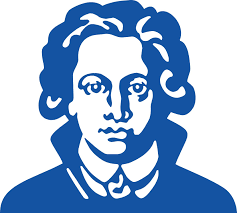
\includegraphics{logo.png}}\\
    {\bigskip}    
    {Sommersemester 2020}\\
}
\author{
    {Jan van Dick}\\
    {Matrikel-Nummer: 6081227}\\
    {Betreuer: Dr. Jonas Heller}
}
\date{\today}

\begin{document}

\maketitle
\frontmatter

\onehalfspacing
\tableofcontents

\mainmatter

\chapter{Einleitung}
So, wie Friedrich Nietzsche in dem Aphorismus vom \qq{[T]olle[n] Menschen}\footfullcite[Vgl.][S. 481. Nachfolgend zitiert als \emph{KSA 3}.]{nietzsche_morgenrote_1999} in \emph{Die fröhliche Wissenschaft} die These vom Tode Gottes entfaltet, enthält sie weit mehr als die bloße Negation Gottes;
indem Nietzsche hinzufügt, dass \emph{wir} ihn getötet haben, gibt sie Zeugnis von der Verantwortung des Menschen für sowohl die Lebendigkeit, als auch die Tötung Gottes: 
Der Mensch hat Gott geschaffen, als dann außer ihm und selbstständig existierend, nur so konnte er ihn töten und damit sich von ihm wieder befreien.\footcite[Vgl.][481]{nietzsche_morgenrote_1999}
Somit liegt eine dialektische Konzeption der Begriffe (zweite) Natur und Befreiung vor, die ich aus der Sicht Nietzsches, sowie der von Christoph Menke rekonstruierten Perspektive Hegels untersuchen möchte.
Beide Begriffe entfalten sich in ihrem Doppelcharakter: zweite Natur als Kritik und Affirmation, Befreiung als Macht und Ohnmacht des Geistes.
In der zweiten Natur schlägt Setzen in Sein um%
\footnote{
    Dass Setzen in Sein umschlägt bedeutet, dass das vom Menschen Gesetzte als Nichtsgesetzes, als Natur, oder \emph{Sein} erscheint\footfullcite[Vgl.][S. 142. Nachfolgend zitiert als \emph{AuB}.]{menke_autonomie_2018}: 
    Der Mensch hat Gott geschaffen, dieser wurde dann zu ihm gegenüber selbständiger seiender Natur. 
}; 
hierin liegt zum Einen die Verwirklichung des Geistes, zum Anderen seine In-Natur-Verkehrtheit.\footcite[Vgl.][145]{menke_autonomie_2018}
Ebenso verhält es sich mit dem Begriff der Befreiung: 
sie ist 1. die \emph{Macht} des Geistes neues hervorzubringen und die scheinbare Notwendigkeit des Bestehenden zu durchbrechen, 
2. aber die \emph{Ohnmacht} des Geistes, da die Befreiung nie abgeschlossen ist; 
sie ist nur Befreiung von der Natur \emph{durch} das Setzen einer neuen, aus welcher der Geist sich dann erneut befreien muss.\footcite[Vgl.][80]{menke_autonomie_2018}
Doch während in Hegels Deutung der Geist in der Befreiung, auf Grund der Endlichkeit des menschlichen Geistes, wieder in Natur verfällt, scheint bei Nietzsche in der Metapher des \qq{offene[n] Meer[es]}\footcite[Vgl.][574]{nietzsche_morgenrote_1999}, die Perspektive vorhanden zu sein, die ewige Wiederholung der In-Natur-Verkehrtheit zu überwinden.
Zugleich bezeichnen Hegel und Nietzsche Freiheit als nicht gegeben: 
Freiheit wird bei beiden so gedacht, dass man sie \glqq nicht nur hat, sondern auch beständig  noch erwirbt und erwerben muss\grqq\footcite[][636]{nietzsche_morgenrote_1999}. 
Mit Adorno ließe sich sagen: Freiheit ist die Befreiung aus der jeweiligen Unfreiheit.\footfullcite[Vgl][227]{adorno_negative_dialektik_2003}
Die Dialektik von Freiheit und Notwendigkeit ist demnach Gegenstand meiner Arbeit, 
die Leitfrage der Arbeit also: \textit{gibt es in Nietzsches Philosophie eine Möglichkeit der Überwindung der Notwendig-in-Natur-Verkehrtheit des Geistes?}
Aus der Position des anfangs erwähnten >>Tollen Menschen<<%
\footnote{
    Ich verwende Spitzzeichen, oder Guillements überall dort, wo ich Anführungszeichen in modalisierender Funktion verwende. 
    D.h insbesondere dort, wo sie \emph{kein} Zitat kennzeichnen.
    Außerdem verwende ich Guillements um deutsche Anführungszeichen innerhalb eines Zitates zu kennzeichnen. 
}
liegt es nahe, diese Möglichkeit in einem Bewusstsein vom Gewordensein der zweiten Natur zu suchen (Gott kann getötet werden, wenn erkannt wird, das er \emph{geschaffen} ist). 
Dies werde ich im Verlauf auch als >>Bewusstsein der Scheinhaftigkeit<< bezeichnen.
Zugleich, muss aber der Schein selbst \qq{mich fühlen lassen, dass hier Schein [...] und nichts mehr ist}\footcite[][417.]{nietzsche_morgenrote_1999}.
Zu fragen wäre demnach, ob dieses Bewusstwerden eine Arbeit des einzelnen Individuums ist, oder ob es aus der Struktur der zweiten Natur selbst hervorgehen kann.\\

Nietzsches Aussage über den Tod Gottes bedeutet der Form-Seite nach die Überwindung der vom Menschen gesetzten zweiten Natur (Gott), der inhaltlichen Seite nach aber, dass der Mensch Gott nicht mehr nötig hat und die Bestimmung des Gesetzes sich aus dem Menschen selbst entwickelt. 
Um also den Begriff der zweiten Natur zu erarbeiten, werde ich im \hyperref[abschnitt_1]{ersten Schritt} zunächst auf den Begriff der Autonomie eingehen, da hier der Versuch, Gesetz und Freiheit zusammen und von Gott gelöst zu denken, seinen Ursprung nimmt. 
Der Begriff der zweiten Natur ergibt sich dann aus Hegels Kritik an Kants Autonomiebegriff.
Hegels Ausweg besteht darin, Freiheit sozial zu verstehen.\footfullcite[Vgl.][49]{pinkard_paradox_2019}
Aus dieser Perspektive werde ich Hegels Begriff der Sittlichkeit als soziale Teilhabe entwickeln (a).
Hier wird sich das Paradox der Autonomie in dem Begriff der Gewohnheit wiederholen.
Diese Wiederholung des Paradox werde ich anhand des Begriffs des \qq{geistigen Mechanismus} erläutern, in welchem die Gewohnheit sich als \qq{geistig oder frei} und \qq{mechanisch oder unfrei}\footcite[Vgl.][145]{menke_autonomie_2018} ergibt (b).
Schließlich soll der Begriff der zweiten Natur in der Dialektik von Fall und Verwirklichung des Geistes und dem Doppelcharakter der zweiten Natur als Kritik und Affirmation seinen Abschluss finden (c).
Darin ergibt sich die Grenze des von Menke erarbeiteten Begriffs der Befreiung:
Macht und Ohnmacht der Befreiung -- Freiheit und Unfreiheit bleiben untrennbar miteinander verbunden.

Durch die Hinzunahme Nietzsches soll versucht werden, über diese Grenze hinauszugehen.
Dazu soll in einem \hyperref[abschnitt_2]{zweiten Schritt} gezeigt werden, dass bei Nietzsche ein ähnlicher Begriff der zweiten Natur aufgezeigt werden kann.
Zunächst soll der Begriff der zweiten Natur anhand von Nietzsches Begriff des \textit{Scheins} erläutert werden (a).
Die Befreiung aus dem (sog.) Schein wird darauffolgend in der Unterscheidung des Schauspielers und der Rolle aufgegriffen (b). 
Abschließend sollen beide Begriffe nochmals in dem Absatz über den >>Tollen Menschen<< analysiert und zusammengebracht werden (c).

Im \hyperref[abschnitt_3]{dritten Abschnitt} soll versucht werden, das Problem der Befreiung aus der zweiten Natur zu erläutern, da das >>Wie<< dieser Befreiung, im Vergleich zur Befreiung aus der ersten Natur, bei Hegel und Menke, und letztendlich auch bei Nietzsche, uneindeutig bleibt.

Im vierten und \hyperref[abschnitt_4]{letzten Schritt} werde ich abschließend anhand der Diskussion um das \qq{offene Meer}, zur Beantwortung der Leitfrage kommen, d.h. die Frage beantworten, ob und inwiefern es bei Nietzsche eine Möglichkeit der Überwindung der ewigen Wiederholung der Befreiung geben kann. 
Es wird sich schließlich ergeben, dass zwar in Nietzsches Konzeptionen auf diese Befreiung über die Befreiung hinaus hingedeutet wird, diese aber auch bei Nietzsche nicht verwirklicht ist.


\chapter{Hauptteil}

Es sei hier ein Zitat Nietzsches vorangestellt, auf welches ich am Ende der Arbeit eingehen werde, aus dem sich aber zunächst einige zentrale Begriffe für die weitere Beschäftigung mit dem Thema \emph{Zweite Natur und Befreiung} ergeben:

\begin{itemize}
    \item[] \textelp{} so finden wir als reifste Frucht an ihrem [der Sittlichkeit] Baum das \so{souveraine} \so{Individuum}, das nur sich selbst gleiche, das von der Sittlichkeit der Sitte wieder losgekommene, das autonome übersittliche Individuum (denn \qq{autonom} und \qq{sittlich} schliesst sich aus) \textelp{} \footfullcite[][S. 293. Nachfolgend zitiert als \emph{KSA 5}. Hervorhebung im Original. Sofern nicht anders vermerkt, sind im Verlauf alle Hervorhebungen im Original.]{nietzsche_jenseits_2014}
\end{itemize}

\subsubsection{Aus der Natur hervorgehen und sich von ihr unterscheiden}
Zunächst spricht Nietzsche im selben Abschnitt von der Sittlichkeit als eine \qq{\so{vorhistorische} Arbeit}\footcite[][293]{nietzsche_jenseits_2014}.
Diese Sittlichkeit beschreibt Nietzsche als die Entwicklung des Menschen, in der er sich durch Zurichtung und Gewohnheit von seiner Natur befreit, die aber zugleich der Freiheit gegenübersteht, weil sie eine neue Form von inneren Zwang schafft (\qq{der Mensch [muss] \textelp{} \emph{notwendig} geworden sein}\footcite[][292]{nietzsche_jenseits_2014}).
Darum ist die \qq{reifste Frucht} der Sittlichkeit dasjenige Individuum, welches sich von ihr wieder befreit.
Dies erinnert stark an Hegels Begriff des Geistes, der dadurch bestimmt ist \qq{aus der Natur herzukommen und sich von der Natur zu befreien}\footfullcite[][S. 294. Nachfolgend zitiert als \emph{LdF}.]{khurana_freiheit_2017}.
Nach Thomas Khurana ist Geist nicht \emph{einmal} aus der Natur hervorgegangen, sondern tut dies immer wieder auch in den höheren Stufen des Geistes.\footcite[Vgl.][294]{khurana_freiheit_2017}
Wenn Geist wesentlich die Bewegung seiner Befreiung aus der Natur ist, dann ist die Frage, \emph{welche} Natur es ist, aus der er sich immer wieder befreit. 
Es ergibt sich daraus, dass der Geist durch seine eigene Bestimmung zur Natur zurückgeführt wird und dass die Natur aus der er sich befreit, letztendlich eine Natur ist, die er sich selbst voraussetzt: zweite Natur.\footcite[Vgl.][320]{khurana_freiheit_2017}
Genau das meint Nietzsches Rede vom Vorhistorischen: 
der Geist hat sich von der Natur befreit, indem er seine eigene (zweite) Natur, gesetzt hat.
Das Nicht-Mehr-Vorhistorische ist, sich auch von dieser wieder zu befreien.
Dadurch hat Freiheit auch bei Nietzsche explizit prozesshaften Charakter. 
Wie in der Einleitung bereits angedeutet, liegt hier die Leitfrage meiner Arbeit: \emph{inwiefern kann dieser Prozess aufhören und zu einem Ende kommen?}
Nietzsche spricht diesen Ausweg ganz konkret an. 
Er spricht vom \qq{Ende des ungeheuren Prozesses} und vom \qq{übersittliche[n] Individuum}, als Ergebnis dieses Prozesses.\footcite[][293]{nietzsche_jenseits_2014} 
Schließlich wird sich ergeben, dass auch bei Nietzsche der übersittliche Mensch seine Autonomie nicht \emph{hat} und der Prozess nicht schlicht zu einem Ende kommen kann:
gerade das Im-Prozess-Begriffen-Sein bedeutet Freiheit, während ein vorgestelltes Ende für Nietzsche -- wie für Hegel -- ihre Aufhebung wäre.\todo[noline]{Papa fragen}
\\

\subsubsection{Sittlichkeit als Kontrast zur Autonomie}
Meine Arbeit wird von dem Begriff der Autonomie ausgehen. 
Hier werde ich zunächst das Paradox, in welches sich die Autonomie verstrickt, und dann den Ausweg in der Sittlichkeit beschreiben.\todo[noline]{Papa fragen}
Nietzsche hingegen bestimmt Autonomie als den Schritt über die Sittlichkeit \emph{hinaus}:
Autonomie ist insofern der Anfang und das Ende des Prozesses.
Nietzsche definiert Sittlichkeit als die \qq{\so{herk"ommliche} Art zu handeln und abzuschätzen}%
\footnote{
    \cite[][22]{nietzsche_morgenrote_1999}. 
    Nietzsche verweist im oben zitierten Abschnitt explizit auf diese Stelle der Morgenröte.
}%
, zu welcher der Mensch durch Disziplinierung erst kommen muss.
Nur durch diese >>Bildung<< kommt der Mensch zu den \qq{>>guten Dinge[n]<<}\footcite[][297]{nietzsche_jenseits_2014}. 
So ist auch bei Hegel Sittlichkeit als handelnde Verwirklichung des Guten\footfullcite[Vgl.][§ 142, S. 161. Nachfolgend zitiert als \emph{Rph}.]{hegel_grundlinien_2017} definiert.
Und auch zu ihr kommt der Mensch nach Hegel nur durch Bildung\footcite[Vergleiche dazu etwa:][§ 187 A, S. 191]{hegel_grundlinien_2017}.
Nietzsche bewertet Sittlichkeit allerdings gänzlich anders als Hegel:
Sittlichkeit ist ein notwendiger Schritt zur Freiheit, über den dann aber wieder hinausgegangen werden muss.
Die Autonomie muss, so könnte man sagen, \emph{durch die Sittlichkeit hindurch}.\\

\subsubsection{Kritik: Freiheit als das sich Bestimmende}
Der dritte Aspekt deutet sich genau an dieser Stelle an. 
Während Kants formalistische Definition der Freiheit nach Hegel inhaltsleer bleibt, kann nach diesem Freiheit nicht als reine Unbestimmtheit oder bloße Abstraktion verstanden werden.
Neben dem Moment der bloßen Unbestimmtheit, ist die einfache Bestimmung gleichsam ungenügend, da sie \qq{eben so \so{Negativit"at}, Aufheben [ist] als das erste -- es ist nämlich das Aufheben der ersten abstrakten Negativität}\footcite[][§ 6 A, S. 39]{hegel_grundlinien_2017}.
Khurana drückt dies so aus, dass das Subjekt einer Bestimmung bedarf, die dem Ich einen konkreten Inhalt gibt und selbst die Form des Ich enthält\footcite[Vgl.][285]{khurana_freiheit_2017}. 
Freiheit ergibt sich erst in der Einheit dieser beiden Momente und Freiheit des Willens ist eben das: sich \qq{in Einem, sich als das Negative seiner selbst, nämlich als \so{bestimmt}, \so{beschr"ankt} zu setzen und bei sich, d.i. in seiner \so{Identit"at} mit sich und Allgemeinheit zu bleiben}\footcite[][§ 7, S. 40]{hegel_grundlinien_2017}.\\

\subsubsection{Bei-Sich-Sein-im-Anderen}
Hieraus kommt Khurana auf Hegels Formel des \qq{Bei-Sich-Selbst-Sein-im-An\-de\-ren}%
\footnote{
    \cite[][283]{khurana_freiheit_2017}.
    Ich verwende hier und im Folgenden diese >>kompakte<< Formulierung Khuranas, welche inhaltlich aus §§5-7 der Rechtsphilosophie Hegels stammt.
}.
Das Setzen der Bestimmtheit geschieht nämlich, wie im obigen Zitat erläutert, \qq{in Einem}, in dem \qq{Negativen seiner selbst} und dieses ist nach Khurana \emph{Natur}. 
Genauer: die vom Geist selbst gesetzte, \emph{zweite} Natur.
Damit können wir den Bogen zurück zum ersten Aspekt schlagen: 
indem das Subjekt Natur setzt, ist es in der Natur bei sich; das ist Sittlichkeit.
Obwohl Nietzsche diesen Aspekt zu unterschlagen scheint, fasst er das Problem und auch die \emph{Möglichkeit} der zweiten Natur mit Hegel richtig auf: 
sie ist Kritik und Affirmation zugleich.
Wie die Dialektik von Kritik und Affirmation zu denken, Nietzsche über die endlose Wiederholung der Befreiung hinausgeht und welche Probleme bei ihm und bei Hegel im Laufe der Entwicklung auftreten, darum wird es im Folgenden gehen.

\section{Zweite Natur bei Hegel}\label{abschnitt_1}
Ein Versuch, Freiheit als diese Einheit von Freiheit und Bestimmung zu verstehen, ist der Begriff der Autonomie. 
Um den Begriff der Autonomie einzuführen und zu beschreiben, wie Hegel und Menke sich auf ihn beziehen, werde ich zunächst in Kürze auf Kants Versuch eingehen, das Paradox der Autonomie aufzulösen.
Der Begriff der Autonomie, wie Kant ihn erarbeitet, nimmt schließlich eine positiven Realisation der Freiheit an.\todo[noline]{Nachschlagen: AuB}
Freiheit jedoch so zu verstehen, dass man sie beständig noch erwerben muss\footcite[Vgl.][636]{nietzsche_morgenrote_1999}, bedeutet, Freiheit als Befreiung zu verstehen, also als einen Akt, der noch (oder immer wieder) geschehen muss, als einen Akt der Negation.
Kants Ansatz, Freiheit als \emph{eigene} Gesetzgebung zu bestimmen, ist der Versuch, diesen Akt der Negation zum Verschwinden zu bringen\footcite[Vgl.][53]{menke_autonomie_2018}.
Zugleich ist es der Versuch, das Paradox der Autonomie aufzulösen.
Hegels Kritik der Autonomie versucht hingegen aufzuzeigen, dass sich dieses Paradox in der Selbstgesetzgebung auch bei Kant erneut wiederholt.
Ich möchte zunächst anhand von Hegels Kritik der Autonomie den Begriff der Sittlichkeit erarbeiten.
Aus diesem komme ich zur Gewohnheit, aus welcher sich das erneute Auftreten des Paradox in der Sittlichkeit ergibt.
Schließlich werde ich die sich entfaltende Dialektik von Geist und Mechanismus, sowie Kritik und Affirmation beschreiben und daraus die Begriffe zweite Natur und Befreiung erarbeiten und an ihnen den Ausweg aus dem Paradox skizzieren.

\subsection{(a) Autonomie und Sittlichkeit}
Der Tod Gottes hat bei Nietzsche, wie in der Einleitung bereits erwähnt, nicht bloß die Bedeutung der Befreiung aus der zweiten Natur, sondern ist ebenso eine Reflexion auf die Umwälzung innerhalb der (Moral-)Philosophie seines und des vorangegangenen Jahrhunderts. 
Waren doch die Gesetze der Moral durch Gott und die Freiheit als die Befolgung dieser göttlichen Gebote bestimmt, so entzieht die Überwindung Gottes diese Gesetze der außer dem Menschen liegenden Macht.
Der Tod Gottes beginnt deshalb auch dort, wo die Moral nicht mehr bloß durch ihn bestimmt ist. 
Der Begriff der Autonomie versucht nun zweierlei: 
er versucht die Bestimmung der Moral von Gott zu lösen und in den Menschen zurückzuführen, ohne jedoch den Schritt hinter Gott zurückzutreten und Freiheit durch blindes Bestimmt-Sein durch die Natur, die sinnlichen Triebfedern, zu sehen: nicht in dem blinden Folgen meiner sinnlichen Triebe, sondern in dem Handeln nach dem \emph{selbst gegebenem} Gesetz bin ich frei.
\footnote{
    \cite[Vgl.][19]{menke_autonomie_2018},
    bzw. \fullcite[][8]{khurana_paradox_2019}.
}
Autonomie bedeutet nach Menke, dass freies Wollen und verpflichtendes Sollen in eins fallen.
Allerdings ist die Selbstgesetzgebung nur als heteronom zu denken:  
entweder folgt die Selbstgesetzgebung aus einem anderen, äußeren Gesetz (äußere Heteronomie) oder beruht auf der freien Willkür des Subjekts (innere Heteronomie) -- das bezeichnet das >>Paradox der Autonomie<<.\footcite[Vgl.][S. 19 - S. 20.]{menke_autonomie_2018}

Kants Versuch, das Paradox aufzulösen besteht darin, den Fokus von \emph{Selbst}\-Gesetzgebung zu \emph{eigener} Gesetzgebung zu verlegen, wodurch es kein Wählen eines vorhandenen Gesetzes ist, sondern ein Gesetz des Subjekts selbst.\footcite[Vgl.][22]{menke_autonomie_2018}
Dabei bestimmt sich das Gesetz, indem das Subjekt seine Maxime so wählt, dass es zugleich wollen kann, \qq{dass sie zu einem allgemeinen Gesetz werde}\footfullcite[][51. Nachfolgend zitiert als \emph{Gms}.]{kant_kritik_2014}. 
Statt sich ein Gesetz zu geben, gibt das Subjekt \qq{seinen Trieben die \emph{Form} des Gesetzes}\footcite[][24]{menke_autonomie_2018}; das Gesetz erhält dadurch allgemeinen Charakter.%
\footnote{
    \cite[Vgl.][65.]{kant_kritik_2014} 
    Auf Ähnliche Art und Weise beschreibt Hegel das Gute als die Einheit des besonderen und des Allgemeinen Willens.\footcite[Vgl.][§ 129, S. 134.]{hegel_grundlinien_2017}
    Diese Einheit des objektiven und subjektiven Moments bildet ebenso die Bestimmung der Sittlichkeit.
}
Autonomie ist durch die Freiheit der Wahl der Maxime, wie die Freiheit ebenso durch das Gesetz bestimmt, denn die Kausalität des freien Willens ist \qq{die Eigenschaft des Willens, sich selbst ein Gesetz zu sein}\footcite[][81]{kant_kritik_2014}.
Damit ist bei Kant das erreicht, was ich als Bestimmung der Autonomie aufzeigte: 
das normative Gesetz ist zurück beim Menschen und obliegt nicht einer äußeren Macht (Gott), zugleich wird Freiheit nicht verstanden als blindes Unterliegen der sinnlichen Triebfedern. 
Nach Hegel wiederholt sich hier das Paradox der Autonomie, da die Allgemeinheit des Gesetzes nur durch die \emph{Form} bestimmt ist und selbst inhaltsleer bleibt:
es \qq{bleibt damit nur die abstrakte Allgemeinheit [...] oder das abstrakte \emph{Positive}, dass Bestimmungslose zu ihrer Bestimmung} und Kants Autonomieformel verkommt zum \qq{leeren Formalismus}.\footcite[][§ 135, S. 139.]{hegel_grundlinien_2017}
Kant geht mit seiner Verschiebung von Selbst- zu eigener Gesetzgebung und durch die Erhebung des Subjektiven zur objektiven Allgemeinheit, einen entscheidenden Schritt in Richtig Hegel, der Formalismus seines moralischen Freiheitsbegriffs zeigt sich aber, indem sich hier das Paradox wiederholt, als noch ungenügend.\\

Worin genau besteht nun Hegels Ausweg aus dem Paradox?
Die Kritik Hegels, an Kants Begriff der Autonomie, hat seinen Grund auch in dem, was ich als notwendige Verknüpfung von Abstraktion (Bestimmungslosigkeit) und Bestimmung (sich einen Inhalt geben), nannte.%
\footnote{
    \cite[Vgl.][§ 7, S. 40.]{hegel_grundlinien_2017}, oder auch: oben S. 6.
}
Freiheit kann letztendlich nur dort herrschen, wo dieser Doppelcharakter verwirklicht ist.
Dieser Doppelcharakter drückt sich in der Sittlichkeit aus, welche Hegel beschreibt als 
\begin{itemize}
    \item[] die Idee der Freiheit, als das lebendige Gute, das in dem Selbstbewusstsein sein Wissen, Wollen und durch dessen \textit{Handeln} seine Wirklichkeit, sowie dieses an dem sittlichen Sein seine an und für sich seiende Grundlage und bewegende Zwecke hat [...]\footcite[][§ 142, S. 161. Hervorhebung von mir]{hegel_grundlinien_2017} 
\end{itemize}
Auch bei Kant ist das allgemeine Gute (formal) durch das subjektive Wollen bestimmt,
und auch bei ihm existiert der Begriff der Handlung.%
\footnote{
    \qq{\emph{handle} stets nach derjenigen Maxime von der du zugleichen wolle kannst, dass sie ein allgemeines Gesetz werde}\footcite[][S. 51. Hervorhebung von mir.]{kant_kritik_2014}.
}
Allerdings bestimmt sich nach Hegel, ob diese oder jene Handlung gut ist, nur durch das \qq{Wissen [und] Wollen} des einzelnen Subjekts.
Indem dies nach Hegel ein nur gedachter Prozess ist, ist die Entscheidung darüber stets \qq{sowohl fähig wahr, als bloße \so{Meinung} und \so{Irrtum} zu sein}\footcite[][§ 132 A, S. 136]{hegel_grundlinien_2017}.
Nach Hegel können Handlungen nicht als die, des auf sich allein gestellten Individuums gesehen werden:
vielmehr ist \emph{jede} Handlung bei Hegel immer schon im sozialen Kontext gedacht und von ihm abhängig, denn:
\qq{sie hat an dem sittlichen Sein [...] ihre Grundlage}.
Zu beurteilen, ob eine Handlung gut oder schlecht ist, bedeutet sie als eine Handlung innerhalb einer sozialen Praxis zu verstehen.\footcite[Vgl][28]{menke_autonomie_2018}
Einfach gesprochen, ist eine soziale Praxis nichts anderes, als eine für eine bestimmte Gruppe an Individuen gemeinsame Art und Weise nach bestimmten Regeln zu handeln.
Beurteilt wird also gemäß diesen \emph{Regeln} der sozialen Praxis und diese sind nichts als der gemeinsame Konsens der Teilnehmenden: 
eine Handlung ist Teil einer Praxis, \qq{genau dann, wenn die Gemeinschaft sie als solche aufnimmt}\footfullcite[][65]{brandom_paradox_2019}.
Verstehe ich mich beispielsweise als einen Fußballspieler und nehme den Ball in die Hand und werfe ihn in das Tor, ist die Entscheidung darüber, ob diese Handlung gemäß den Regeln des Fußballspiels gut oder mangelhaft ist, von nichts abhängig, als der Anerkennung, oder Nicht-Anerkennung der anderen Teilnehmenden der Praxis des Fußballspiels.\footnote{
    Unter Umständen wäre es genauer dies als die Funktion des Schiedsrichters zu sehen, der von den Teilnehmenden die Funktion, die Praxis zu regulieren, zugewiesen bekommen hat. 
    Im Falle eine Fußballspiels auf dem Bolzplatz ist allerdings nicht mal dieser nötig.
}
Dem folgend, werden Urteile nach Menke gefällt, insofern sowohl Gegenstand als auch Autor des Urteils Teil einer (sozialen) Praxis sind\footcite[Vgl.][28]{menke_autonomie_2018}, bzw. sich als Teil verstehen (wollen). 
Und sie \qq{erfolgen mit Bezug auf die Gesetze [...] die eine Praxis ausmachen; die also das jeweilige Gute spezifizieren}\footcite[][S. 28 - S. 29]{menke_autonomie_2018}.
Das >>Gute<< und was die Praxis ist, ihre Regeln (bzw. Gesetze), sind also ein und dasselbe und zugleich die Regeln des Teilnehmers der Praxis -- er folgt \qq{seinem eigenen Gesetz}.%
\footnote{
    \cite[][29]{menke_autonomie_2018}.
    Dies ist sein eigenes Gesetz, aber erst, wenn er sich die Regeln der Praxis angeeignet hat\footcite[Vgl.][32]{menke_autonomie_2018}.
    Dieser Prozess der Aneignung ist einer, der auch in der Bildung und Disziplinierung geschieht.
    (Man stelle sich beispielsweise ein Kleinkind vor, welches Fußballspielen will und ständig den Ball in die Hand nimmt o.ä. während seine Mutter es korrigieren muss. 
    Dieser Prozess, ist der notwendige Prozess der Bildung/ Disziplinierung, durch den das Gesetz zum Gesetz des Subjekts erst wird, an deren Ende es schließlich auch Ausdruck seines Wesens ist.\footcite[Vgl.][§ 147, S. 162]{hegel_grundlinien_2017})
}
Das Gute ist somit kein >>Sollen<<, sondern es ist in der Praxis schon wirklich, denn wie die Handlung an dem sittlichen Sein seine Grundlage hat, ist dieses in jener wirklich.
Von der Seite der Teilnahme gedacht, ist so zu verstehen, inwiefern das Gute zu seinem Inhalt kommt: 
im Gegensatz nämlich zum \qq{abstrakten Guten} (bei Kant), ist das \qq{objektiv Sittliche [...] durch die Subjektivität \so{konkrete} Substanz}\footcite[][§ 144, S. 161.]{hegel_grundlinien_2017}:
das Gesetz der Praxis konstituiert sich durch die Handlungen der Subjekte innerhalb der Praxis.
Der Inhalt kommt somit nicht von außen dazu, sondern er \emph{ist} bereits.
Menke drückt dies auch so aus, dass das Gesetz überhaupt erst Verbindlichkeit besitzt, wenn es existiert und zwar \qq{nicht nur gesollt, sondern schon wirklich ist}\footcite[][57]{menke_autonomie_2018}.

Dies Gesetz hat \qq{eine [...]  unendlich festere Autorität und Macht, als das Sein der Natur}\footcite[][§ 146, S. 164.]{hegel_grundlinien_2017}.
Unter diesem Gesetz, dieser neuen Autorität, erfährt das Subjekt zugleich die Befreiung von den bloßen Naturtrieben.\footcite[Vlg.][§ 149, S. 164]{hegel_grundlinien_2017} 
Indem das objektive Gesetz nun sozial, oder geistig bestimmt ist, befreit sich das Subjekt von der unmittelbaren Natur, ist aber zugleich dieser neuen Autorität unterworfen. 
Dies kann, um einen ersten Bogen zu Nietzsche zu schlagen, an dem Beispiel Gottes verdeutlicht werden: 
indem der Mensch Gott, genauer: eine Gottesfiktion, durch sein Handeln (Beten, zur Kirche Gehen, etc.) schafft, schafft er ihn als ein Gesetz, welches das der Natur ersetzt. 
Wie ja wirklich die Macht der Natur durch Gott aufgehoben und dieser für z.B. Naturkatastrophen, verantwortlich gemacht wird.
Zugleich gibt Gott den Menschen Gesetze, die (mit eingehender Naturbeherrschung) für den Menschen tatsächlich eine \qq{unendlich festere Autorität und Macht} besitzen.%
\footnote{
    \fullcite[Vgl.][33]{adorno_dialektik_der_aufklärung_1981}.
    Auf das Motiv Gottes, als das Setzen einer ersten zweiten Natur, werde ich mich noch einige Male beziehen. 
    Ich lasse hier grundsätzlich die mir ansonsten sehr einleuchtende Spezifizierung Khuranas aus, in welcher er drei Stufen unterscheidet, in denen das Hervorgehen aus und das Setzen der Natur sich wiederholt: Anthropologie, Phänomenologie und Sittlichkeit.
    Erst die dritte dieser Stufen stellt die Sittlichkeit, als \qq{der zur \emph{vorhandenen Welt} und \emph{zur Natur des Selbstbewusstseins gewordene Begriff der Freiheit}} (\cite{hegel_grundlinien_2017}, § 142, S. 161) dar.
    Nur auf diese beziehe ich mich hauptsächlich, während ich die anderen Stufen in meinen Ausführungen größtenteils auslasse, oder zusammendenken werde. 
    Es ist nämlich gleichfalls so, dass diese Stufen nicht bloß nebeneinander stehen, sondern z.B. \qq{die Form der Gewohnheit [...] alle Stufen des Geists} (\cite{khurana_freiheit_2017}, S. 401) betrifft.
    Khurana unterscheidet von der Sittlichkeit 1. die Anthropologie, in der der Geist mittels der Gewohnheit aus seiner noch in Natur versenkten Form sich befreit und 2. die Phänomenologie, in welcher der Geist sich seiner selbst bewusst wird (\cite{khurana_freiheit_2017}, S. 394 - S. 397).
    Die Schaffung Gottes, ist demnach eher in der ersten oder zweiten Stufe zu suchen, als in der Sittlichkeit. 
    Um den Rahmen der Arbeit allerdings nicht zu sprengen, verweise ich hier nur auf diese Unterscheidungen und nutze Gott als ein allgemeines Beispiel, denn was damit aufgezeigt wird, trifft auf alle Stufen in gleicher Weise zu. 
}
In der sozialen Teilnahme an einer Praxis, und das ist das Entscheidende, konstruiert das Subjekt jedoch nicht nur das Gesetz, als ein ihm äußerliches, es ist \qq{dem Subjekt nicht ein \so{Fremdes}, sondern es gibt das \so{Zeugnis des Geistes} von ihnen als von \so{seinem eigenen Wesen}}\footcite[][§ 147, S. 162.]{hegel_grundlinien_2017}.
Die Gesetze stehen dem Subjekt also 1. nicht fremd gegenüber, da sie durch seine eigene Handlung gesetzt sind und aus dem selben Grund konstituieren sie 2. das Subjekt, da es seine eigenen autonomen Handlungen sind;
es wird konstituiert \qq{durch eben die Gesetze, die die Praxis konstituieren}\footcite[][30]{menke_autonomie_2018}.

Sittlichkeit und soziale Teilhabe so verstanden, scheinen das Paradox der Autonomie aufzulösen, denn die Gesetze sind hier sowohl inhaltlich bestimmt, als auch frei gesetzt.%
\footnote{
    Ich verweise an dieser Stelle bereits darauf, dass Hegel den Moment, in welchem \qq{das Sittliche die wirkliche Lebendigkeit des Selbstbewußtseins ist}, als \qq{Verhältnis-lose Identität}\footcite[][§ 147 A, S. 163.]{hegel_grundlinien_2017} beschreibt. 
    Von diesem Punkt aus ist es schwer, sich eine Transformation des Bestehenden vorzustellen.
    Wie diese Transformation, oder die Befreiung in der Sittlichkeit zu denken ist, werde ich im \hyperref[abschnitt_3]{dritten Abschnitt} diskutieren.
}\\

Wie kehrt nun das Paradox in der Sittlichkeit zurück? 
Wie oben bereits in der Analogie zu Gott erwähnt, schafft der Mensch in der Sittlichkeit sich Gesetze, die zwar 1. das Paradox der Autonomie aufheben, d.h. sie sind eigene, inhaltlich bestimmte und zugleich Wesens-konstituierende Gesetze, aber sie werden 2. zu einer Macht, die noch die Macht der Natur überbietet in der Autorität über den Menschen.
D.h. das Schaffen (oder Setzen) von Gott, gibt den Menschen die Moral, aber versklavt ihn zugleich einer neuen, inneren Notwendigkeit: \qq{das Sittliche [erscheint] als eine \emph{zweite Natur}}.%
\footnote{\cite{hegel_grundlinien_2017}, § 151, S. 166.
    Wie hier der Begriff des \qq{Erscheinens} zu verstehen ist, ist mir etwas unschlüssig. 
    Als Lesart schlage ich vor, dass Hegel so verstanden werden muss, dass Sittlichkeit als zweite \emph{Natur} (nicht als \emph{zweite} Natur) erscheint. 
    Und sie \emph{erscheint}, weil es \emph{zweite}, vom Menschen gesetzte Natur ist, darum, denke ich, spricht Hegel von \emph{Erscheinen} nicht von \emph{Sein}.
    Auf ähnliche Art und Weise schreibt Menke später: \qq{[d]as Gesetzte wird als Nichtgesetztes gesetzt}\footcite[][142]{menke_autonomie_2018}, und meint damit eben das \emph{Erscheinen} des Gesetzten als Natur.
    Würde sie übrigens, damit greife ich auf \hyperref[abschnitt_2]{den zweiten Abschnitt} vor, als \emph{zweite} Natur erscheinen, wäre in gewissermaßen erfüllt, was Nietzsche fordert: 
    dass der Schein mich spüren lässt, dass er Schein und nichts weiter ist\footcite[Vlg.][416.]{nietzsche_morgenrote_1999}.
}

Im Gegensatz zu Kant, bei dem die moralisch verstandene Befreiung des Mensch den Bruch mit der äußeren Notwendigkeit (Triebe, natürliche Determination etc.) bedeutet, kann bei Hegel die Befreiung nur darin liegen, die äußere Notwendigkeit, bzw. die Macht der ersten Natur, zu ersetzen durch eine geistig selbst hervorgebrachte Notwendigkeit.
Darum schreibt Hegel, die verwirklichte Freiheit ist aus dem Menschen hervorgebracht als eine \emph{zweite Natur}.\footcite[Vlg.][§ 4, S. 34.]{hegel_grundlinien_2017}
Der Mensch kann demnach nur frei sein, indem er eine Form der Verknüpfung schafft, die nicht geistig, sondern \emph{natürlich} ist. 
Menke beschreibt dies als die \qq{\emph{eigene} natürliche Verfassung des Geistes}, in der aber \qq{das Werden seiner Autonomie}\footcite[][40. Hervorhebung von mir]{menke_autonomie_2018} erst entstehen kann.
Die Hervorbringung dieser natürlichen Verfassung ist Grundbedingung und Ergebnis von Sittlichkeit und Befreiung.
Einen ähnlicher Gedanke findet sich auch bei Nietzsche. 
Er schreibt, dass es nach dem Tod Gottes \qq{noch Jahrtausende lang Höhlen geben [wird], in denen man seinen Schatten zeigt. -- Und wir -- wir müssen auch noch seinen Schatten besiegen!}\footcite[][467]{nietzsche_morgenrote_1999}
Nietzsche beschreibt mit den Schatten die vom Menschen gesetzten Notwendigkeiten, die auch nach der Befreiung aus der (ersten) Natur noch bestehen. 
In der Metapher des Sonnenuntergangs, als vollständiger Zerfall alles Bestehenden, beschreibt Nietzsche allerdings zugleich die Gefahr, dass es \emph{keine} neue Formen von (natürlichen) Verknüpfungen geben wird.%
\footnote{
    Die Sonnenfinsternis beschreibt Nietzsche als Folge von Zerstörung, Zerfall und Unbestimmtheit, welcher der wieder freie Horizont gegenübersteht. 
    Die absolute Abstraktion, die \qq{Zertrümmerung aller bestehenden gesellschaftlichen Ordnung}\footcite[][§ 5 A, S. 39.]{hegel_grundlinien_2017} ist, wie wir schon in der Einleitung zu Hegels Freiheitsbegriff gesehen haben, auch bei Nietzsche problematisch und hängt eng zusammen mit dem Problem der zweiten Natur.
    Es deutet sich hier also bereits an, dass die Konzeption des \qq{übersittlichen} Menschen, wenn man Nietzsches gesamtes Werk in Betracht zieht, nicht so eindimensional sein kann, wie zuerst angenommen.
    Wie Sonnenfinsternis, Schatten und offenes Meer genauer verstanden werden müssen, werde ich im \hyperref[abschnitt_2]{zweiten Abschnitt} erläutern.
}
Es muss die vom Geist selbst hervorgebrachte Notwendigkeit, die \emph{zweite} Natur (die Schatten) geben, von der wir uns dann erneut befreien müssen.
Damit bedeutet Befreiung nicht nur die Befreiung aus der ersten, sondern ebenso die Befreiung aus der zweiten Natur. 

In diesem Sinn ist auch zu verstehen, was es für Hegel heißt, Freiheit als \qq{Reflexion des Geistigen in sich, seiner Unterscheidung von dem Natürlichen und seinem Reflexe auf dieses}\footcite[][§ 194 A, S. 197.]{hegel_grundlinien_2017} zu verstehen: 
Geist bestimmt sich, wie zu Beginn des Hauptteils bereits gesehen, wesentlich dadurch: 
aus der Natur zu kommen und sich \emph{immer wieder} von ihr zu unterscheiden, sich permanent aus dieser zu befreien -- sei es von der Natur als erste Natur oder von der eigenen natürlichen Verfassung.
Wir haben also die in sozialen Praktiken geistig produzierte, zweite Natur einerseits selbst als das Mittel der Befreiung von der Natur zu verstehen, zugleich aber als das, wodurch sich die In-Natur-Verkehrtheit \emph{im Geist} wiederholt.\footcite[Vgl.][41]{menke_autonomie_2018}
In diesem Sinne tritt hier das Paradox der Autonomie in der Sittlichkeit als Dialektik und Wechselwirkung zwischen Befreiung und zweiter Natur auf.
Diese innere Dialektik der Befreiung und der zweiten Natur werde ich im Folgenden mit Menke als die Dialektik der Gewohnheit beschreiben.

\subsection{(b) Gewohnheit - Dialektik von Geist und Mechanismus}
Wir konnten bisher sehen, dass sich in der Teilnahme an sozialen Praktiken, das objektive Sittliche auf eine Art und Weise konstituiert, dass es einerseits durch die Handlungen inhaltlich bestimmt ist und andererseits für die Subjekte nicht äußerlich bleibt, sondern gewissermaßen das \emph{eigene} Gesetz ist. 
Diese Identität von subjektiver Individualität und objektiver Sittlichkeit erscheint, wie wir weiter gesehen haben, als zweite Natur.
Hegel schreibt: \qq{das Sittliche erscheint, als die allgemeine Handlungsweise derselben - als \so{Sitte}, - die \so{Gewohnheit} desselben als \so{zweite Natur}}\footcite[][§ 151, S. 166]{hegel_grundlinien_2017}.
Die angesprochene Wieder-in-Natur-Verkehrtheit des Geistes erklärt Hegel also ausgehend von der Gewohnheit.
Daher werde ich im Folgenden anhand der Gewohnheit, nahe an Menkes Analyse, die innere Dialektik der zweiten Natur versuchen zu beschreiben.
Dabei ist es zentral die Gewohnheit, wie sich in Menkes Begriff des \qq{geistige[n] Mechanismus}\footcite[][145]{menke_autonomie_2018} bereits andeutet, selbst in dem Spannungsverhältnis von Freiheit und Unfreiheit zu betrachten. 
Gewohnheit ist nach Menke zum Einen das Ergebnis von Bildung (also geistige Tätigkeit) und ermöglicht, indem sie uns von der bloßen naturmäßigen Verknüpfung befreit, erst Freiheit.
Zum Anderen ist sie zugleich selbst eine Form natürlicher Verknüpfung und damit äußerlicher Notwendigkeit: 
sie macht den Menschen \qq{einerseits frei, [...] doch andererseits zu ihrem \emph{Sklaven}}\footnote{\fullcite[][§ 410 Z, S. 189. Nachfolgend zitiert als \emph{Enz}.]{hegel_enzyklopädie_1969}, zitiert bei \cite[][127]{menke_autonomie_2018}}.
Nicht nur sind in der Gewohnheiten zwei scheinbar unvereinbare Seiten enthalten, Menke beschreibt sie außerdem als zentrale Gestalt des Geistes, die sowohl den Beginn des Geistes ausmacht, und sich ebenso fortwährend in allen Stufen des Geistes wiederfindet; 
der Geist kommt über sie nicht hinaus, sondern \qq{bleibt wesentlich Gewohnheit}\footcite[][129]{menke_autonomie_2018}.

\begin{comment}
Während Khurana Gewohnheit wesentlich ausgehend von dem Werden des Geistes beschreibt und sie deshalb vor allem den elementaren Stufen des Geistes zuordnet, macht auch dieser deutlich, dass Gewohnheit eine allumfassende Seinsweise des Geistes ist, die sich nicht nur auf den elementaren Stufen, sondern auch in der Sittlichkeit zeigt.\footcite[Vgl.][433]{khurana_freiheit_2017}\todo{Im Falle von Kürzungsnotwendigkeit weglassen}
\end{comment}

Menke erklärt den Begriff \qq{geistige[r] Mechanismus} daraus, dass die Handlungsweise der Gewohnheit 1. unbewusst, also im \emph{Vollzug} der Handlung \qq{nicht durch Gründe geleitet} und 2. \qq{kein bloß äußerlich determiniertes, kausal erklärbares Geschehen} \footcite[][128]{menke_autonomie_2018} ist.
Wie kann diese scheinbare Unvereinbarkeit aufgelöst werden?
Ich habe oben bereits angedeutet, dass Menke die Gewohnheit als Ergebnis des Prozesses der Bildung beschreibt.
So beschreibt Hegel 1. die Gewohnheit dadurch, dass sie ein solches Ergebnis eines geistigen Prozesses ist, selbst als \emph{geistig}. 
\begin{comment}
Dem füge ich noch hinzu, dass sie nicht nur auf Grund des geistigen Prozesses, der Einwohnung, sondern eben dadurch geistig ist, dass der Prozess selbst aus Gründen angeeignet wurde, so beschreibt Menke, die Teilnahme an der sozialen Praxis, als eine Teilnahme \emph{aus Gründen}.
Menke beschreibt den Prozess der Bildung, als die \qq{>>Einwohnung<< eines künstlichen Zwecks}\footcite[][129]{menke_autonomie_2018}.
\end{comment}
Andererseits ist 2. der Geist in ihr wieder zurückgekehrt in eine bloß natürliche Verfassung: 
die Elemente der Gewohnheit sind \qq{in bloß äußerlicher Notwendigkeit}\footcite[][129]{menke_autonomie_2018} verknüpft, daher ist sie \emph{mechanisch}.
Auf diese beiden Seiten werde ich nun etwas näher eingehen.\\

\subsubsection{1. Die Gewohnheit ist geistig}
Dass die Gewohnheit uns frei macht, ist am besten so zu verstehen, dass sie uns \emph{befreit}. 
Sie befreit uns nämlich von dem bloß natürlichen Sein unseres Körpers.
Musik ist ein gutes Beispiel dafür. 
Ohne durch Gewohnheit das Notenlesen einstudiert, die Verknüpfung der Töne mit den Tasten des Klaviers und den Positionen meiner Finger eingeübt zu haben, bin ich nicht, frei Klavier zu spielen.% 
\footnote{
    Das Musikbeispiel ist deshalb interessant, weil hier deutlich wird, inwiefern die Musiker*in 1. immer wieder Gewohnheiten entwickeln muss (jedes neue Können muss Gewohnheit geworden sein) und 2. müssen sich gerade frei improvisierende Musiker*innen immer wieder auch von ihren Gewohnheiten befreien (z.B. von gewohnten Tonlagen, oder bekannten Rhythmen) und dies tuen sie letztendlich nur \emph{durch} die Ausbildung neuer Gewohnheiten\footfullcite[Vergleiche dazu auch:][189]{hegel_religion_1986}.
}
Durch Übung und \emph{Eingewöhnung} wird mein Körper in Besitz von Fähigkeiten gebracht, die mir dann als Möglichkeiten zur Verfügung stehen.
Durch Gewohnheit distanziere ich mich einerseits von meinen natürlichen, und setze andererseits neue und eigene Bestimmungen. 
Es ist demnach \qq{[d]ie wesentliche Bestimmung [der Gewohnheit] die \emph{Befreiung}}\footcite[][§ 410 A, S. 185]{hegel_enzyklopädie_1969}.
In diesem Sinne beschreibt Menke die Gewohnheit als \qq{Praxis einer ontologischen Transformation}\footcite[][130]{menke_autonomie_2018}:
das natürliche Sein, welches mich bestimmt, transformiert sich auf eine Art und Weise, dass mein Körper nun mir zum Instrument wird.
Hier wird ersichtlich, dass die durch Gewohnheit erworbenen Fähigkeiten nicht von Natur aus da sind, vielmehr muss ich meinen Körper erst dazu \emph{bilden}.\footcite[Vgl.][§ 410 Z, S. 190]{hegel_enzyklopädie_1969}
Die Gewohnheit ist somit eine künstliche und erworbene, dadurch \emph{geistige} Fähigkeit.
Dem ist in Anschluss an Khurana noch hinzuzufügen, dass durch die Gewohnheit, der Geist sich im und durch den Geist vergegenständlicht und ihm dadurch in der objektiven Welt ein Mittel zur Verfügung steht, mit dem er seine Zwecke verwirklichen kann, ohne sich selbst der Gewalt der Natur auszusetzen.\footcite[Vgl.][426]{khurana_freiheit_2017}
Dies zeigt eindrücklich, inwieweit die Gewohnheit notwendig ist für die Freiheit des Geistes.

Sie ist aber nicht nur in ihrem Resultat geistig, indem sie dem Geist bestimmte Verhaltensweisen ermöglicht, sondern auch der Prozess ihrer Aneignung ist als geistiger zu verstehen.
Betrachten wir jedenfalls die Gewohnheit in der Sittlichkeit, dann ist die Praxis selbst, aus der die Gewohnheit folgt, eine Praxis, die \emph{aus Gründen} angeeignet wurde.
Menke beschreibt, erst in der Einheit des Subjekts mit dessen Praxis, erst in der Sittlichkeit, kann von ihm als einer \qq{Instanz des Handelns aus Gründen}\footcite[][29]{menke_autonomie_2018} gesprochen werden.
Also die Gewohnheit, die ich mir in der Praxis aneigne, ist auch selbst eine aus Gründen angeeignete und somit geistig. 
Es ist eine \qq{willentlich ausgeführte Bewegung}, die durch die Einübung zur \qq{bewusstlos Gewollten} wird.\footcite[][414]{khurana_freiheit_2017}
Das bestimmt die Zwecke der Gewohnheiten für Hegel letztlich als \qq{Zwecke des Geistes} und die Gewohnheiten selbst als \qq{Kunstwerk der Seele}\footcite[][131]{menke_autonomie_2018}.\\

\subsubsection{2. Die Gewohnheit ist mechanisch}
Eine erste Erklärung für das Mechanische an der Gewohnheit ist, dass die Handlungen \emph{automatisch} ausgeführt werden.%
\footnote{
    Kein Musiker muss sich noch beim Spielen eines Tons darauf konzentrieren ihn zu spielen, wie er es im Prozess des Lernens getan hat. 
    Das Spielen selbst geschieht automatisch.
}
Diese Erklärung, Gewohnheit sei Automatismus, bleibt jedoch oberflächlich.\footcite[Vgl.][132]{menke_autonomie_2018}
Menke beschreibt, dass alle Fähigkeiten egal welcher Art immer \qq{die logische Form einer Besonderung des Allgemeinen}\footcite[][132]{menke_autonomie_2018} haben. 
Gerade geistige Handlungen zeichnen sich nach Menke dadurch aus, dass Handlung \emph{in der} Situation ausgeführt werden.
Und zwar auf eine Art und Weise, dass das Wahrnehmen der Situation Teil des Ausübens ist.\footcite[Vgl][132]{menke_autonomie_2018} 
Das Wissen, welches zum Ausüben gehört, ist also einerseits das allgemeine Wissen von der Fähigkeit und andererseits das, der besonderen Situation: \qq{[e]s ist Wissen \emph{vom} Allgemeinen \emph{im} Besonderen}\footcite[][133]{menke_autonomie_2018}.
Diese beiden Seiten des Wissen interagieren auf eine Weise, dass \qq{das allgemeine Wissen [...] in der -- nicht: auf die -- Wahrnehmung der besonderen Situation angewandt wird.}\footcite[][133]{menke_autonomie_2018}
Menke beschreibt nun weiter, dass es der Gewohnheit genau an dieser Interaktion des Besonderen und Allgemeinen Wissens mangelt:
die Gewohnheit ist \qq{nur die aus der \emph{Wiederholung vieler Einzelheiten} durch \emph{Reflexion} hervorgebrachte \emph{abstrakte} Allgemeinheit}\footcite[][§ 410 Z, S. 188]{hegel_enzyklopädie_1969}.
Es mangelt der Gewohnheit also nicht an Allgemeinheit, sondern an Wahrnehmung des Besonderen, dadurch wiederholt sich in der Gewohnheit stets dasselbe:
Sie kann nur der allgemeinen Regel \emph{folgen} und diese nicht \emph{anwenden}. 
Dadurch aber \qq{ist das Selbst der Gewohnheit weder von außen noch von innen determiniert, sondern es ist frei, denn es will.}\footcite[][134]{menke_autonomie_2018}.
Dies macht auch Khurana deutlich, indem er die Gewohnheit als abstrakte Allgemeinheit beschreibt, welche von den Unterschieden im Einzelnen absieht.\footcite[Vgl.][431]{khurana_freiheit_2017}
Die sich hieraus ergebende mechanische Gestalt der Gewohnheit führt letztendlich dazu, dass Gewohnheit Gefahr läuft, nicht nur selbst natürliche Verknüpfung zu sein, sondern den Geist \qq{in Natur zurückschlagen zu lassen}\footcite[][430]{khurana_freiheit_2017};
darin liegt letztlich die Gefahr, dass die Gewohnheit \qq{der Tod selbst ist}\footcite[189]{khurana_freiheit_2017}.\\

Um an dieser Stelle noch einen kleinen Bogen zu Nietzsche zu schlagen, lässt sich hiervon ausgehend verstehen, was Nietzsche damit meint, dass er die kurzen Gewohnheiten, als eine Abwehr gegen das Verfallen in Abstumpfung und Interessenlosigkeit, am meisten liebt.
Die \qq{\so{dauernden} Gewohnheiten} dagegen \qq{hasst} er: \qq{meine Lebensluft [..] \so{verdickt}} sich.\footcite[][535]{nietzsche_morgenrote_1999}
Schließlich ist für ihn \qq{das eigentlich Fürchterliche} aber \qq{ein Leben ganz ohne Gewohnheiten}\footcite[][535]{nietzsche_morgenrote_1999}.
Auch für Nietzsche stehen Gewohnheiten daher in einem vertrackten Verhältnis zwischen Befähigung und Freiheit einerseits und Stumpfheit und Unfreiheit andererseits. 
Auch für ihn sind sie eine Notwendigkeit des Geistes, die sich auch in den höheren Stufen des Geistes nicht überwinden lässt. 

\subsection{(c) Dialektik von Kritik und Affirmation}\label{kritik_affirmation}
Menke greift auf Marx Unterscheidung von dogmatischer und \qq{wahrhaft philosophischer} Kritik zurück, nach der die dogmatische mit ihrem Gegenstand \qq{kämpft} oder ihm ihren Gegensatz äußerlich gegenüberstellt, während die wahrhafte Kritik ihn in ihrer inneren \qq{Antinomie}\footfullcite[][296]{marx_kritik_1977} begreift, und Menke teilt anhand dieser Unterscheidung die Kritik der zweiten Natur in eben diese Seiten:
sie beschreibt 1., wie der Geist in der zweiten Natur im Widerspruch zu seinem eigenen Begriff steht, und 2., dass zweite Natur die \emph{Selbst}verstellung \emph{des} Geistes und damit Ausdruck eben dieser inneren Antinomie ist.
Wir hatten am Beispiel der Gewohnheit gesehen, inwieweit zweite Natur die Wiederholung der Natur im Geist ist. 
Da der Geist aber seinem Begriff nach nichts ist, als \qq{die Wirklichkeit der Freiheit}\footcite[][137]{menke_autonomie_2018}, erscheint die zweite Natur als eine Selbstverstellung des Geistes und steht im Widerspruch mit dem Begriff des Geistes:
zweite Natur ist der \qq{Tod des Geistes durch den Geist und im Geist}\footcite[][43]{menke_autonomie_2018}.
Hier deutet sich bereits die zweite Seite an:
es ist der Tod des Geistes \emph{durch} den Geist.
Die Naturverkehrtheit des Geistes wird nicht nur beschrieben, sondern auch aus dem Begriff des Geistes immanent erklärt;
sie wird erklärt als \emph{Selbst}verstellung \emph{des} Geistes. 
Die Kritik der zweiten Natur ist also kritisch gegen den Geist selbst, nicht nur gegen die mangelhafte Form, die dieser in ihr annimmt, und erklärt zugleich den Geburtsakt der mangelnden Form des Geistes -- und ihn als Geburtsakt durch den Geist.%
\footnote{
    Insofern bestimmt Menke die Kritik der zweiten Natur im Verlauf auch als genealogische Kritik.
}
Menke zeigt weiter auf, dass die zuvor beschriebene Kritik an der Gewohnheit einen anthropologischen Ursprung hat und erklärt aus der folgenden anthropologischen Bestimmung zwei Seiten des endlichen Geistes, mit denen das Problem der zweiten Natur eine neue Bedeutung erhält.
Dies möchte ich im Folgenden näher erläutern.\\

Dass die Wiederholung der Natur im Geist etwas Anthropologisches ist, bedeutet, dass die Selbstverkehrung des Geistes in Erscheinung tritt, auf Grund der endlichen Gestalt des menschlichen Geistes.%
\footnote{
    Hegel drückt dies in der Enzyklopädie recht humorvoll aus: \qq{Ungewohntheit und lange Fortsetzung des Denkens macht Kopfweh} (\cite[][§ 410 A, S. 186]{hegel_enzyklopädie_1969}).
}
Zweite Natur ist gleichermaßen mangelhaft und unvollständig, wie der Geist des Menschen endliche und menschliche Gestalt hat.
Dies bedeutet zweierlei: 
1. kann die Kritik der zweiten Natur in der menschlichen Gestalt, auf Grund seiner Endlichkeit niemals überwunden werden;
der Mensch unterliegt notwendig der Wiederholung der Natur,
2. schafft die Bestimmung des Geistes als Grund für seine eigene Naturverfallenheit eine neue Perspektive: 
indem der Geist Grund für seinen Fall zurück in die Natur ist, \emph{unterliegt} er diesem nicht nur, er bringt ihn selbst hervor.
Diese Form genealogischer Kritik, die die Erklärung der Hervorbringung mit erläutert, zeigt, dass \qq{der Geist [..] immer schon  mehr als der endliche Geist [ist], in den er sich verkehrt}\footcite[][140]{menke_autonomie_2018}.
Dieses Mehr-als-endlicher-Geist ist nach Menke \emph{absoluter Geist}, kann aber als \emph{Grund} für die Selbstverkehrung des endlichen Geistes nicht \emph{Jenseits} des endlichen Geistes liegen.\footcite[Vgl.][140]{menke_autonomie_2018}
Damit nimmt der Begriff der zweiten Natur eine eigentümliche Weichenstellung zwischen endlichem und absolutem Geist ein:
Während der \emph{endliche} Geist in der zweiten Natur durch die Selbstverkehrung bestimmt ist, vollzieht der \emph{absolute} Geist aus Freiheit seine Selbstverkehrung in die zweite Natur:
\qq{[e]s ist daher das eigene Bewegungsgesetz des absoluten Geistes, in den endlichen Geist zu fallen}\footcite[Vgl.][140]{menke_autonomie_2018}.

Diese eigentümliche Zwischenstellung lässt sich mit dem Begriff \qq{Manifestation des Geistes}\footcite[][140]{menke_autonomie_2018} verstehen. 
Doch was meint Manifestation des Geistes?
Zunächst kann das so verstanden werden, dass der Geist sich in der Natur manifestiert, also, dass der Geist seine Welt, (d.h. das von ihm Hervorgebrachte) setzt als Natur: der Geist offenbart sich (in der Natur), er vergegenständlicht sich.\footcite[Vgl.][143]{menke_autonomie_2018}
Ich hatte zu Begin beschrieben, dass Geist wesentlich Freiheit ist, dass es sich aber um eine Form der Freiheit handelt, die nicht bloße Negativität, sondern ebenso \emph{Bestimmtheit} ist, eine Form der Bestimmtheit, die dem Ich einen konkreten Inhalt gibt.
Diese Form von Bestimmtheit, ließ sich mit Hegel auf die Formel des \qq{Bei-sich-Sein-im-Anderen} bringen.
Wir können nun die Manifestation des Geistes als eben diese Bestimmtheit sehen, durch die das Allgemeine sich besondert, aber dennoch Allgemeines bleibt und zur Identität mit sich selbst kommt.
Das bedeutet, dass es bei der gesuchten Form der Bestimmtheit nicht um diesen oder jenen Inhalt gehen kann, den der Geist sich gibt, sondern, dass es die Bewegung des Geistes, sich in der Natur zu offenbaren, selbst ist, die diesen Inhalt ausmacht. 
Hegel beschreibt dieses Offenbaren weiter, als \qq{\emph{Setzen} der Natur als \emph{seiner} Welt; ein Setzen, das [...] zugleich \emph{Voraussetzen} der Welt als selbstständiger Natur ist.}\footcite[][§ 384, S. 29]{hegel_enzyklopädie_1969} 
In dem selbst gesetzten Sein kommt das Ich zu seiner Bestimmtheit, in der es \emph{bei sich} ist; zugleich ist dies Gesetzte \emph{selbstständige} Natur, und darum ist er bei sich \emph{im Anderen}.

Hegel zeigt in dem oben angeführten Zitat zwei verschiedene Operationen auf: 
das Setzen der Natur als Welt, sowie das Voraussetzen der Welt als Natur.
Jenes ist als \emph{Aneignung}, dieses als \emph{Verselbstständigung} zu verstehen.\footcite[Vgl][141]{menke_autonomie_2018}
Es handelt sich aber keinesfalls um zwei verschiedene, sondern vielmehr um ein und dieselbe Operationen: 
das Setzen von Sein, welches zugleich beides hervorbringt.
Zweite Natur bezeichnet genau diese doppelte Bedeutung: 
sie bezeichnet 1. als \emph{zweite} Natur das \qq{geistige Gesetztsein des selbstständig Seienden} und 2. als zweite \emph{Natur} \qq{das Selbstständigsein [...] des durch den Geist Gesetzten}\footcite[][142]{menke_autonomie_2018}.
Aber es sind eben keine zwei voneinander getrennten Momente, zweite Natur ist nicht einmal als \emph{zweite} Natur und einmal als zweite \emph{Natur}, sondern sie ist \emph{zweite Natur}.
Ebenso wenig ist das Setzen von Sein in diese zwei Momente zu unterteilen:
das Voraussetzen ist ein Setzen, weil das vom Geist Hervorgebrachte als Natur gesetzt wird,
ebenso muss das \qq{Setzen der Natur als seiner Welt} ein Voraussetzen sein, weil das was gesetzt wird sonst nicht Natur wäre: 
\qq{das Gesetzte wird als Nichtgesetztes gesetzt}\footcite[][142]{menke_autonomie_2018}, also als Natur \emph{voraus}gesetzt, nur so kann es Aneignung von \emph{Natur} sein.%
\footnote{
    Der Begriff der zweiten Natur als Kritik aufgefasst, entlarvt genau dieses Verhältnis: er zeigt auf, dass das als Nichtgesetztes Gesetzte, Gesetztes ist.
    Als Affirmativ aufgefasst, zeigt er die Macht des Geistes, Gesetztes als Nichtgesetztes zu setzen.
}
In diesem Sinne ist zweite Natur die Selbstverwirklichung des Geistes, weil das Setzen, ursprünglich rein begrifflich, das tatsächliche Erschaffen von Natur ist, aber das Erschaffene \emph{des Geistes}.
Diese Form der Selbstverwirklichung des Geistes ist die andere Seite der zweiten Natur: es ist die \emph{Affirmation} der zweiten Natur, die Affirmation des Geistes.\footcite[Vgl.][143]{menke_autonomie_2018}\\

Ich hatte im vorherigen Absatz versucht aufzuzeigen, dass das Mehr, welches der endliche Geist enthält, eigentlich das ausmacht, was Hegel den absoluten Geist nennt.
Indem der Geist im Setzen von Sein \qq{die \emph{Affirmation} und \emph{Wahrheit} seiner Freiheit sich gibt}\footcite[][§ 384, S. 29]{hegel_enzyklopädie_1969}, \emph{ist} \qq{[d]er absolute Geist zweite Natur}\footcite[][144]{menke_autonomie_2018}.
Zweite Natur ist also gerade darin affirmativ, dass sie in ihrer Form die Struktur des absoluten Geistes enthält: 
\qq{das vom Geist gesetzte [muß] zugleich als ein unmittelbares Seiendes gefaßt werden. 
Dies geschieht [...] auf dem Standpunkt des \emph{absoluten} Geistes.}\footcite[][§ 385 Z, S. 34]{hegel_enzyklopädie_1969}
In der (affirmativen Seite der) zweiten Natur ist die Einheit von Setzen und Sein zusammen gedacht, dies macht den entscheidenden Unterschied zum endlichen Geist aus: 
dort fallen die beiden Seiten auseinander.\footcite[Vgl.][S. 143 - S. 144]{menke_autonomie_2018}
Endlicher Geist ist zugleich \qq{Sein \emph{gegen} Setzung [...] und Sein \emph{durch} Setzung}\footcite[][144]{menke_autonomie_2018}.
In diesem Sinne ist der endliche Geist bestimmt von dem Widerspruch zwischen Begriff und Wirklichkeit. 
Während im absoluten Geist Setzen und Sein als Einheit zusammenfallen, erscheint diese im endlichen Geist stets als Setzung \emph{oder} Sein, weil etwas in der Realität niemals zugleich als Natur \emph{und} geistig hervorgebracht ist.%
\footnote{
    Interessant ist, um nochmals einen kleinen Bogen zu Nietzsche zu schlagen, dass nach Nietzsche zweite Natur, bzw. Schein ebenso diese Einheit von Setzen und Sein darstellen soll.
    Nach ihm ist Schein 1. Natur selbst und lässt sich 2. anmerken, dass er nur Geist ist.\footcite[Vgl.][S. 417]{nietzsche_morgenrote_1999}. 
}
Menke schlussfolgert schließlich: 
\qq{Endlicher Geist zu sein heißt, absoluter Geist gewesen zu sein.
Aber ebenso notwendig heißt absoluter Geist zu sein, endlicher Geist zu \emph{werden}}.\footcite[][144]{menke_autonomie_2018}
Einerseits bedeutet dies, dass im endlichen Geist die Affirmation des Geistes enthalten ist.
Andererseits wird hier deutlich, dass wenn die Affirmation darin besteht, dass der Geist \emph{Natur} setzt, das Gesetzte auch als Sein erscheinen muss.
Dies kann es aber nur im endlichen Geist.
Gewissermaßen kann also der absolute Geist seine eigene Setzung nur im endlichen Geist verwirklichen, da nur dort das Gesetzte als Nichtgesetztes erscheint.
Damit, so müsste konsequent gefolgert werden, liegt die Einheit von Setzen und Sein auch dem absoluten Geist nicht vor. 
%Damit gilt allerdings auch für den absoluten Geist, dass die Einheit von Setzen und Sein ihm nicht vorliegt.


\subsection{Zwischenfazit und Problembestimmung}\label{zwisschenfazit}
Wir sind ausgegangen von der Kritik der Autonomie, und haben eine erste Rettung der Freiheit im Begriff der Sittlichkeit erarbeitet. 
Als das lebendige Gute kommt das objektiv Sittliche und das Individuelle in der Teilhabe an einer sozialen Praxis zusammen. 
Dadurch konnten Gesetz und Freiheit zusammen gedacht, oder als durcheinander bestimmt gesehen werden, ohne inhaltsleer zu bleiben.
Zugleich zeigte sich im Begriff der zweiten Natur, genauer: der Gewohnheit, die Wiederholung des Paradox der Autonomie.
Gewohnheit ist einerseits \emph{geistig}, da sie durch Bildung willentlich angeeignet (ein Setzen) ist, aber indem sie zur bloßen Wiederholung, zum \emph{Mechanismus} wird, ist sie  Ausdruck von Unfreiheit.
Unter Hinzunahme der Dialektik von Verwirklichung und Fall des Geistes, muss dieses Verhältnis allerdings ergänzt werden:
der Umschlag von Setzen in Sein beschreibt nicht bloß kritisch den Fall, sondern zugleich affirmativ die Verwirklichung des Geistes.
Dabei ist die affirmative Seite notwendig auf die kritische bezogen: 
die Verwirklichung ist nur dort möglich, wo der Geist sich in Natur verkehrt.
Menke beschreibt, dass der Freiheitsverlust zugleich die Selbstüberschreitung, bzw., dass diese nur durch jenen ist\footcite[Vgl.][145]{menke_autonomie_2018}.
Es sind somit beide Seiten der zweiten Natur, die kritische und die affirmative, untrennbar miteinander verbunden, allerdings nach Menke \qq{zugleich einander strikt entgegengesetzt}\footcite[][147]{menke_autonomie_2018}.
Untrennbar verbunden sind sie, indem die Verwirklichung des Geistes nur im Fall der Geistes möglich ist.
Strikt voneinander getrennt sind sie aber, in den Übergängen von endlichen in absoluten und absoluten in endlichen Geist, weil sie sich gegenseitig \emph{bekämpfen}:
die Natur verschlingt die Welt des Geistes und reißt sie in die ewige mechanische Wiederholung, während die neue Welt die Wiederholung aufbricht, unterbricht und neue Sinnzusammenhänge schafft.\footcite[Vgl.][147]{menke_autonomie_2018}
So beschreibt Menke die affirmative Seite der zweiten Natur nicht als positiv, sondern gleichfalls als negativ und zerstörerisch:
sie affirmiert nicht das Bestehende (denn das ist die Wiederholung der Gewohnheit, welche sie ablehnt), sondern dessen Aufbrechen: 
die Affirmation ist als >>neue<< \qq{die Zerstörung der \emph{falschen} zweiten Natur}%
\footnote{
    \cite[][S. 148. Hervorhebung von mir.]{menke_autonomie_2018}
    Diese Zerstörung bezeichnet Menke auch als \qq{das plötzliche Hervortreten des Werkes, des Gedanken, der Tat}, welches \qq{die immer gleiche Wiederholung der abstrakt imaginärer Identitäten [bekämpft]}\footcite[][147]{menke_autonomie_2018}.
}%
, und daher nicht positiv, sondern negativ.
Damit sind Kritik und Affirmation jeweils auf positive und negative Weise affirmativ bzw. kritisch:
die Affirmation ist 1. positiv die Kraft des Geistes Sein zu Setzen und 2. negativ die Zerstörung, oder besser: 
Unterbrechung der Wiederholung. 
Die Kritik ist 1. negativ die Verurteilung der Wiederholung der Natur in der Gewohnheit, sogleich umfasst sie 2., qua Negation, positiv den Willen der Überwindung des Falls des Geistes.\\

Es findet sich bei Hegel also kein Ausweg aus der ewigen Wiederholung der Befreiung, bzw. der In-Natur-Verkehrtheit des Geistes:
nicht nur ist die Befreiung ohne die Schaffung einer zweiten Natur nicht möglich, auch ist ohne die Wiederholung von Natur Freiheit nicht denkbar.%
\footnote{
    Im einen Fall gibt es Freiheit >>eine Zeit lang<<, bis sie sich dann in Natur verkehrt, während im zweiten Fall die Freiheit selbst \emph{nichts anders bedeutet}, als das Natur-Werden des Gesetzten, denn nur dort ist der Geist bei sich im Anderen.
}
Im nächsten Abschnitt werden wir einige Stellen aus Nietzsches Werken betrachten, um die Möglichkeit der Überwindung der Wiederholung bei Nietzsche zu untersuchen.
Im Anschluss an die eben geführte Debatte, wollen wir bei Nietzsche Ausgang nehmen, von der Dialektik der zweiten Natur, bzw. der Dialektik des Scheins (denn so wird uns der Begriff bei Nietzsche begegnen).
Diese Dialektik drückt sich nochmals zusammengefasst und auf Nietzsche bezogen so aus, dass der Schein einerseits Natur sein soll (damit die Kraft des Geistes, Natur zu setzen, verwirklicht ist), andererseits geistig sein soll, damit der Geist nicht wieder in Natur verfällt. 
Wir werden bei Nietzsche in der Betrachtung des Scheins und des Schauspielers, das Problem von der objektiven, wie von der subjektiven Seite aus erfahren. 

\section{Zweite Natur bei Nietzsche}\label{abschnitt_2}
Bevor ich mich Nietzsche annähere, seien noch einige Worte zu der Frage >>wie Nietzsche lesen?<< gesagt.
Mir ist wohl bewusst, dass die Rezeption Nietzsches sich schwierig gestaltet, da er nicht nur vom Nationalsozialismus und Denkern dieser Tradition angeeignet wurde, sondern auch innerhalb der Linken umstritten ist.
Umstritten scheint mir beispielweise die Annäherung Nietzsches an (links) idealistische Positionen, welche Paul Stephan als die Nietzsche am wenigsten zuordenbare Strömung bezeichnet.\footfullcite[Vgl.][S. 26. Nachfolgend zitiert als \emph{LN}.]{stephan_nietzscheanismus_2019}
Stephan stimmt, indem er Tucholsky zitiert%
 \footnote{
    \qq{Sag mir, was du brauchst, und ich will dir dafür ein Nietzsche-Zitat besorgen.} (\fullcite[][]{tucholsky_gesammel_1975} Zitiert bei \cite[][17]{stephan_nietzscheanismus_2019})
},
darin überein, dass es schwierig ist Nietzsche eine Hauptlehre zu unterstellen, da es ihm oft an Eindeutigkeit fehlt, hält aber dagegen, dass diese Uneindeutigkeit bewusst gesetzte Methode ist.\footcite[Vgl.][18]{stephan_nietzscheanismus_2019}
Was Nietzsche mit Sicherheit wollte, war: \emph{sich sein Werk für einen selbst fruchtbar zu machen}. 
Das heißt: Nietzsches Gedanken nicht zu erstarrten Metaphern werden zu lassen, sondern sie für die Metaphern im eigentlichen Sinne zu nehmen -- mit denen sich dann auch \emph{spielen}, oder genauer: >>tanzen<< lässt.

In Anschluss an die Leitfrage, soll in diesem Abschnitt der Grundstein für die Möglichkeit der Befreiung aus der Befreiung gelegt werden.
Dabei hatte ich zu Beginn der Arbeit angedeutet, dass diese dritte Befreiung eine Tat des Individuums sein, oder in den objektiven Verhältnissen liegen könnte. 
Die Frage nach dem Schein, sowie die des Schauspielers, stehen für die Betrachtung des Problems von der subjektiven, individuellen und der objektiven, sittlichen Seite. 
Diese beiden Seiten möchte ich schließlich in dem bereits zitierten Aufruf des >>Tollen Menschen<<: \qq{Gott ist tot und wir haben ihn getötet!} zusammenbringen und damit am Ende zu unserem Ausgangspunkt zurückkehren. 


\subsection{(a) Was bedeutet Schein?}
Nietzsche mag als Dynamit und Hammer und Zerstörer von Wahrheit und Metaphysik\footcite[Vgl.][59]{stephan_nietzscheanismus_2019} gelten: 
\begin{itemize}
    \item[] die Wahrheiten sind Illusionen, von denen man vergessen hat, dass sie welche sind, Metaphern, die abgenutzt und sinnlich kraftlos geworden sind, Münzen, die ihr Bild verloren haben und nun als Metall, nicht mehr als Münzen in Betracht kommen.\footfullcite[][S. 881. Nachfolgend zitiert als \emph{KSA 1}.]{nietzsche_geburt_1999}. 
\end{itemize}
Aber was bedeutet es für Nietzsche genau, dass die Wahrheit eine bloße Illusion ist? 
Was bedeutet es, dass unsere Begriffe und Namen für die Dinge ihrem Wesen fremd sind?
-- Das Wort \emph{Metapher} weißt bereits auf mehr als die bloße Zerstörung von Wahrheit hin. Denn, dass etwas eine Metapher ist, deutet immer auf einen Zusammenhang zwischen dem Ding und der Metapher und die Metapher schafft zugleich für das Ding eine neue Bedeutung. 
Versteht man Nietzsches Verwendung des Begriffs der Metapher auf diese Weise, dann stellt sich Nietzsches Wahrheitskritik als eine doppelte dar, die einerseits Kritik, andererseits Affirmation ist.\\

Mit der Kritik der Wahrheit, sie sei nichts als \qq{[e]in bewegliches Herr von Metaphern}\footcite[][880]{nietzsche_geburt_1999}, meint Nietzsche mehrere Dinge, auf die ich zunächst einen Blick werfen möchte: 
erstens beschreibt er damit Wahrheit als etwas anthropomorphes, das nicht so in der Welt ist, sondern, was der Mensch erst festlegen musste: er \qq{fixiert, was von nun an >>Wahrheit<< sein soll}\footcite[][877]{nietzsche_geburt_1999}.
Zweitens klingt darin Nietzsches Begriffskritik mit an:
die Wahrheit ist Metapher, also nur abgezogenes Bild von dem eigentlichen Ding, wie der Begriff niemals mit der Sache identisch ist, sondern stets durch \qq{Gleichsetzen des Nicht-Gleichen}\footcite[][880]{nietzsche_geburt_1999} entsteht.
Schließlich betont Nietzsche drittens, dass der Mensch vergessen hat, dass seine Wahrheit immer nur perspektivisch\footcite[Vgl.][364]{nietzsche_jenseits_2014}, nur ein von ihm gemachtes Abbild ihrer ist. 
Dies lässt sich schließlich so zusammenfassen, dass der Mensch nur \emph{glaubt} etwas von den Dingen zu wissen, oder anders: dass er \qq{nach fester Convention [...], unbewusst und nach hundertjährigen Gewöhnungen}\footcite[][881]{nietzsche_geburt_1999} \emph{lügt}.\\

In der fröhlichen Wissenschaft schreibt Nietzsche, dass es ihm schwer fiel einzusehen, dass \qq{unsäglich mehr daran liegt, \so{wie die Dinge heissen}, als was sie sind}\footcite[][422]{nietzsche_morgenrote_1999}.
Es wirkt als revidiere Nietzsche damit die Begriffskritik seiner Frühwerke.
Dabei gerät jedoch die Doppeldeutigkeit der Metapher aus den Augen und, dass Nietzsche nur ihr \emph{Vergessen} kritisiert, nicht ihre Verwendung im Allgemeinen. 
Wenn Nietzsche schreibt, dass es mehr darauf ankommt, \qq{wie die Dinge heißen, als was sie sind}, dann ist dies eigentlich keine Revision seiner Kritik der Metapher, sondern die Unterstreichung dessen, was mit dem Ausruck \emph{Denken in Metaphern} eigentlich gemeint ist.
Nietzsche betont, dass der Mensch im Kreieren von Metaphern \qq{\so{k"unstlerisch schaffendes} Subjekt ist}\footcite[][883]{nietzsche_geburt_1999}.
Er ist schaffendes Subjekt nicht nur indem er den Dingen (neue) Namen gibt, sondern auch, indem die von ihm geschaffenen Metaphern Wirklichkeit werden: 
\qq{der Schein wird zuletzt immer als Wesen und \so{wirkt} als Wesen.}\footcite[][422]{nietzsche_morgenrote_1999}.
Damit wirkt das vom Menschen Geschaffene letztlich als \emph{Wesen} und es ist demnach bedeutender, \qq{wie die Dinge heißen, als was sie sind}, oder (ursprünglich) waren.

Der Schein enthält für Nietzsche also auf ähnliche Art und Weise ein komplexes Verhältnis, wie die Metapher: 
Schein ist einerseits vom Menschen produziert, geistig und daher nicht unmittelbare, erste Natur, andererseits ist dieser doch das selbstständig Seiende und Wirkende und dadurch \emph{Wirk}lichkeit.
Nietzsche betont, man könne von dem Wesen überhaupt nichts aussagen, als \qq{die Prädicate [sic] seines Scheins}, deshalb ist der Schein nicht \qq{der Gegensatz irgend eines Wesens}\footcite[][417]{nietzsche_geburt_1999}.
Es liegt bei Nietzsche also nahe, dass es überhaupt nichts gibt, als Schein und er schreibt, dass Schein \qq{das Wirkende und Lebende selber} ist und mich wissen lässt, \qq{dass hier Schein und Irrlicht und Geistertanz und nichts Mehr ist}\footcite[][417]{nietzsche_morgenrote_1999}.
Indem der Schein selbst wirkend ist, ist er selbstständig dem Geist gegenüber, indem er seine eigene Natur (Schein zu sein) preisgibt, bekennt er sich, als geistig;
Schein ist zugleich Natur und Geist.
Nietzsche fordert hier also die Paradoxe Einheit von Setzen und Sein, denn diese Einheit ist nicht, wie bei Menke, der Übergang von Verwirklichung in Entwirklichung, sondern sie \emph{ist} zugleich Setzen und Sein und damit Vollendung des Geistes, ohne Fall des Geistes zu sein.
Hinzu kommt, dass Nietzsche dies nicht nur fordert, sondern, dass es sich nach ihm wirklich so verhält.
Während bei Menke die Macht des Geistes, Sein zu setzen, sich nur in der Dialektik von endlichem und absolutem Geist ergeben kann,
ist bei Nietzsche Schein Wesen und Bewusstsein vom Nicht-Wesen-Sein zugleich.
Was wir ausgehend von Hegel und Menke als unauflösbares Ineinander von Verwirklichung und Fall des Geistes annahmen, scheint bei Nietzsche in der Wirklichkeit aufgelöst zu sein. \\

Dieses Wissen von der Scheinhaftigkeit, welches ich im Folgenden als >>Bewusstsein der Scheinhaftigkeit<< bezeichnen werde, stellt die explizite Gegenposition dar, zum \emph{Vergessen} der Illusion und zur \emph{kraftlos gewordenen} Metapher.
Nietzsche beschreibt, dass die ursprünglich anschauliche Metapher sich, gerät der Mensch unter die \qq{Herrschaft der Abstractionen [sic]}, zum Begriff \qq{verflüchtig[t]}.\footcite[][881]{nietzsche_geburt_1999}.
Obwohl also der Schein wissen lässt, dass er Schein ist, scheint es gleichfalls eine subjektive Komponente zu geben, welche den \qq{Geistertanz} erkennen muss.
Diese subjektive Komponente findet sich in Nietzsches Unterscheidung vom Erkennenden \emph{mit} und dem Erkennenden \emph{ohne} Anführungszeichen:
letzterer lebt nur \emph{in} der Welt des Scheines ohne ihr Geschaffen-Sein zu erkennen, während ersterer die Einheit von Setzen und Sein erkennt. 
Nietzsche schreibt, dass der Erkennende ein \qq{Festordner} ist, um \qq{den irdischen Tanz in die Länge zu ziehen} und \so{die Dauer des Traumes aufrecht zu erhalten}\footcite[][417]{nietzsche_morgenrote_1999}.
Der Traum (die Verwirklichung des Geistes, die im >>Erkennenden<< \emph{wirklich} ist) besteht also nur so lange fort, wie der Schein von dem Erkennenden auch für Natur genommen wird. 
Es bilden sich zwei Pole:
auf der einen Seite steht das Verlieren in der Metapher, also das Versinken des Geistes in Natur und die daraus resultierende Hypostasierung des Bestehenden.
Auf der anderen Seite, die völlige Aufhebung alles dessen was ist, die >>Entwertung aller Werte<<, welche beidseitig als Vorläufer*innen des Faschismus gesehen werden können.\footcite[Vergleiche dazu beispielsweise:][S. 61, S. 69]{stephan_nietzscheanismus_2019}.
Beide Seiten fanden sich auch bei Hegel als problematisch:
einerseits verfällt der Geist in Natur, andererseits beutet die bloße Willkür gleichfalls Abwesenheit von Freiheit.%
\footnote{
    Und auch Hegel hat diese Form der Willkür des Zerstörens von allem bestehenden mit den Schrecken der Jakobinerherrschaft vergleichen\footcite[Vgl.][39]{hegel_grundlinien_2017}.
}\\

Ich habe versucht hier die objektive Seite zu beschreiben und wir haben gesehen, wie sie notwendig in die subjektive Seite übergeht und wollen diese im Folgenden näher betrachten.

\subsection{(b) Der Schauspieler und die Rolle}
Die Unterscheidung, des >>Erkennenden<< und des Erkennenden, werde ich anhand von Nietzsches Konzeption des Schauspielers und der Rolle vertiefen. 
Der Erkennende hat sich als der gezeigt, welcher in dem Schein versunken bleibt und ihn für Natur nimmt, während der >>Erkennende<< in dem erkannten Schein dennoch seinen Traum tanzt.\footcite[Vgl.][417]{nietzsche_morgenrote_1999}
Wie der Erkennende den Schein für Natur nimmt, wird \qq{aus der Rolle wirklich Charakter [...], aus der Kunst Natur}\footcite[][595]{nietzsche_morgenrote_1999}.
Wie beschreibt Nietzsche diesen Wandeln?
Für Nietzsche bedeutet Rolle etwas künstlich Geschaffenes, welches die Menschen, zum Beispiel im Zuge ihres Berufes -- aus Zwang oder \qq{anscheinender Freiheit}\footcite[][595]{nietzsche_morgenrote_1999} -- annehmen. 
Dabei vergessen sie bald, dass es sich ursprünglich um eine angenommene, erdachte Rolle handelte und es nur Zufall war, dass sie genau diese, und nicht eine aus unzähligen anderen Rollen >>spielen<<.
Nietzsche erläutert, dass sie sich die Rolle auf Grund ihres \qq{guten Spiels}\footcite[][595]{nietzsche_morgenrote_1999} so aneignen konnten:
sie haben sich selbst so sehr in ihrem eigenen Schein verloren, dass \qq{aus der Kunst Natur} geworden ist. 
Diese Dauerhaftigkeit die aus dem Vergessen der Scheinhaftigkeit entsteht beschreibt Nietzsche als \qq{einen Werth ersten Ranges}\footcite[][595]{nietzsche_morgenrote_1999} und drück damit einerseits aus, dass nur auf Grund dieses Vergessens der Mensch sich so ausbreiten und verwirklichen konnte, andererseits wirkt seine Aussage höchst ironisch, er kritisiert damit also eindeutig die Affirmation des Bestehenden.%
\footnote{
    So ähnlich findet sich die Kritik ja auch im erstarren der Metaphern wieder.
}\\ 

Dem Schauspieler hingegen liegt das gegenteilige Verhältnis zu Grunde: 
er ist derjenige, bei dem \qq{alle Natur aufhört und Kunst wird}\footcite[][596]{nietzsche_morgenrote_1999}.
Der Schauspieler erkennt nach Nietzsche den Schein, oder die \qq{Falschheit}, aber spielt sie \qq{mit gutem Gewissen}\footcite[][608]{nietzsche_morgenrote_1999}.
Der Schauspiel befreit sich von der Natur, die ihn bindet und erschafft einen Schein.%
\footnote{
    Nietzsche betont an dieser Stelle die Verdrängung des \qq{sogenannter >>Charakter[s]<<}\footcite[][608]{nietzsche_morgenrote_1999}.
    Für ihn ist selbst der Charakter nur Schein, nur \qq{sogenannter} Charakter.
    Dies macht eine gewisse Spannung auf, wenn es beispielsweise um Nietzsche Antifeminismus oder Sexismus geht, wo es sehr wohl so wirkt, als unterstelle er Frauen ein >>Wesen<<.
    Stephan schreibt hierzu, dass Nietzsche zwar zugesteht, dass es \emph{kein} \qq{natürliches Wesen} der Frau gibt, sondern, \qq{dass ihr >>Wesen<< Ergebnis ihrer patriarchaler Unterdrückung sei}\footcite[Vgl.][50]{stephan_nietzscheanismus_2019}, sieht darin aber keine Rettung von Nietzsches offensichtlichem Antifeminismus.
    Die Befreiung der Frau aus diesen Verhältnissen scheint Nietzsche vehement abzulehnen.
    Dennoch sind diese Aussagen Nietzsches \qq{seiner philosophischen Grundhaltung nach als experimentelle Erfahrungswahrheiten, nicht als absolute Wahrheiten im metaphysischen Sinn zu verstehen}\footcite[][61]{stephan_nietzscheanismus_2019}.
}
Er tut dies nicht >>einfach so<<, sondern mit \emph{Lust}.
Diese \qq{Lust an der Verstellung} zeigt sich als eine \qq{Macht}\footcite[][608]{nietzsche_morgenrote_1999}, welche sich darauf bezieht die (anscheinende) Natur beiseite zu schieben und sie in Kunst zu verkehren.
Dem Schauspieler liegt somit das Moment des Sich-frei-Machens von der Natur zu Grunde. 
Er durchbricht in seiner Lebensweise den Schein der Notwendigkeit und das ist Befreiung.\footcite[Vgl.][41]{menke_autonomie_2018}.
Der Schauspieler vertritt, was ich als \qq{Bewusstsein der Scheinhaftigkeit} bezeichnete, die einerseits die Notwendigkeit, andererseits die daraus folgende Veränderbarkeit des Scheins erkennt.
Er Unterscheidet sich darin auch vom >>Erkennenden<<, da er dieses Verhältnis nicht nur \emph{erkennt} sondern auch handelnd sich verwirklicht in der Durchbrechung des Bestehenden: 
er \emph{befreit} sich.
Der Schauspieler erkennt also 1. das Verhältnis von Schein und Wesen, gleich dem >>Erkennenden<< und 2. kann seine Lebensweise als die der Befreiung aus der zweiten Natur bezeichnet werden. 
\\

Zuletzt will ich aus diesem Unterschied einen Bogen zurück zur Befreiung schlagen.
Khurana schreibt zur Befreiung des Geistes, dieser \qq{will sich befreien, als die Natur aus sich herausbildend}\footcite[][393]{khurana_freiheit_2017}. 
Hier liegt das Verhältnis der Rolle vor: 
der Mensch setzt die Rolle als seine Natur:
Die geistig geschaffene Rolle \emph{wird} zur Natur. 
Dies ist die eine Seite der Befreiung. 
Die zweite ist der Schauspieler, der sich aus der Natur, der Rolle, die selbst nur zweite Natur, also Schein ist, befreit und stattdessen Kunst und Schein setzt. 
Aber mit dem entscheidenden Unterschied, dass dem Schauspieler seine Rolle nicht selbst wieder als Natur erscheint. 
Bildet damit auch der Schauspieler Natur aus sich heraus, die er (im Gegensatz zur Rolle) als von ihm geschaffen erkennt? 
Ist gerade der Schein, den der Schauspieler ausbildet auch der, der mich selbst wissen lässt, dass er Schein ist?
Wie im vorherigen Abschnitt die objektive in die subjektive, geht hier die subjektive in die objektive Seite über.

\subsection{(c) Gott ist tot!}\label{abschnitt_2_3}
Ich werde nun versuchen die gezeigte subjektive und objektive Seite in der Erzählung des >>Tollen Menschen<< zusammenzubringen.

Nietzsches These vom Tode Gottes, dass >>wir<< ihn getötet haben, ist mehr als bloße Negativität. 
\qq{Müssen wir nicht selber zu Göttern werden}\footcite[][481]{nietzsche_morgenrote_1999}, um ihn getötet zu haben?
Dass der Mensch selbst zum Gott wurde, gibt das Zeugnis der Verantwortlichkeit für sowohl die Lebendigkeit, als auch die Tötung Gottes.
Der Mensch ist Gott geworden, indem er ihn \emph{geschaffen} hat, dadurch nur konnte er ihn töten. 
Gott ist vom Menschen selbst gesetzt, er ist Schein, der sich gegen ihn verselbstständigte, der lebendig und unabhängig vom Menschen existierend wurde, denn nur als einmal lebendig gewesen, kann er auch \emph{ver}wesen \qq{-- auch Götter verwesen!}\footcite[][481]{nietzsche_morgenrote_1999}
Gott ist somit geistiges Produkt des Menschen, in welchem der Geist selbst wieder zur Natur sich verkehrte.
Denn, wie bei Hegel erläutert, ist die Verwirklichung auch der Fall des Geistes.
Das bedeutet hier, dass der Mensch vergessen hat, dass er Schöpfer des Schöpfers war und, dass dieser gegenüber jenem zu einer selbstständigen Macht wurde.
Der Tod Gottes verweist also einerseits auf die Macht des Menschen Sein zu Setzen%
\footnote{
    \qq{Denn tausend Götter muss gebären/ Die Brust, die einen Gott aus sich erschuf}\footfullcite[][146]{lou_im_kampf_2007}. 
    Bei Lou Andreas-Salomé fehlt allerdings die bei Nietzsche mitschwingende Dialektik von Verwirklichung und Entwirklichung.
} 
und ist andererseits die Befreiung aus der In-Natur-Verkehrtheit:
%[d]er Mensch ist für einen Augenblick erneut Gott, er kann Gott töten, er \emph{hat} (nach Nietzsches Erzählung) Gott getötet.
Menke macht jedoch deutlich, dass die Befreiung stets das Schaffen einer neuen zweiten Natur ist. 
Die \qq{plötzlich hervorbrechende Tat}, zerstört die \qq{falsche} zweite Natur, gerade indem sie eine neue setzt.
Ohne dieses neue Setzen wäre die plötzliche Tat nichts als \qq{der Fanatismus der Zertrümmerung}\footcite[][§ 5 A, S. 39]{hegel_grundlinien_2017}.
Bei Nietzsche sind die Folgen der Befreiung nicht so eindeutig.
Der >>Tolle Mensch<< spricht \emph{aus Angst} vor der bloß zerstörerischen Tat: \qq{Was thaten wir, als wir diese Erde von ihrer Sonne losketteten? [...] Müssen nicht Laternen am Vormittage angezündet werden?}\footcite[][481]{nietzsche_morgenrote_1999}
Aber es gibt noch eine zweite Perspektive: 
zwar ist der Tod Gottes für die Einen eine untergegangene Sonne, aber für die Anderen, die \qq{geborene Rästhselrather}, ein \qq{offenes Meer}\footcite[][S. 573 - S. 574]{nietzsche_morgenrote_1999}.
Dies können wir mit dem Schauspieler und der Rolle zusammenbringen. 
Für diese ist der Schein Natur, dass Gott Illusion ist also vergessen, oder nie gewusst. Jede Zerstörung oder Umwälzung ist notwendig eine \qq{Verdüsterung und Sonnenfinsternis}\footcite[][573]{nietzsche_morgenrote_1999}.
Der Schauspieler hingegen weiß, dass es bloß Geistertanz ist, für ihn ist dieser \qq{Blitz und Donner}\footcite[][481]{nietzsche_morgenrote_1999} der Bote der \qq{neuen Morgenröthe}, sie sagen: \qq{jede Wagniss des Erkennenden ist wieder erlaubt, das Meer, \so{unser} Meer liegt wieder offen da, vielleicht gab es noch niemals ein so >>offenes Meer<<}\footcite[][574]{nietzsche_morgenrote_1999}.
Der >>Erkennende<< und der Schauspieler sehen im Tod Gottes die Möglichkeit neue Wörter zu Schaffen und neuen Sinn zu stiften.\footcite[Vgl.][70]{stephan_nietzscheanismus_2019}. 
Für Nietzsche braucht es demnach das \emph{Bewusstsein der Scheinhaftigkeit}, wie es beim >>Erkennenden<< vorliegt, um sich in einer Weise zu befreien, die sich nicht im Nichts verliert, sondern neue, wesensbestimmende Elemente setzt.
Damit können wir die in der Einleitung aufgeworfene Frage, ob die Befreiung bei Nietzsche ein neues Moment \emph{in} der Sittlichkeit hervorbringen kann, welches die Möglichkeit mit sich bringt, die ewige Wiederholung der Befreiung zu durchbrechen, beantworten: 
der Schein enthält stets dieses Moment, wissen zu lassen, dass er Schein ist, aber eben nur \emph{für mich} -- was heißt: nur für den >>Erkennenden<<.%
\footnote{
    So schreibt Nietzsche ja: \qq{Schein ist für mich das Wirkende und Lebende selber, dass so weit in seiner Selbstverspottung geht, \emph{mich} fühlen zu lassen, dass hier Schein und Irrlicht und Geistertanz und nichts Mehr ist, -- dass unter all diesen Träumenden auch ich, der >>Erkennende<<, meinen Tanz tanze [...]}\footcite[][S. 417, Hervorhebung von mir]{nietzsche_morgenrote_1999}.
}

\section{Was heißt Befreiung aus der zweiten Natur}\label{abschnitt_3}
Befreiung bedeutet >>Durchstoßen des Scheins der Notwendigkeit<<\footcite[Vgl.][41]{menke_autonomie_2018}.
Bei Nietzsche ist uns die Befreiung im Schauspieler begegnet, der sich von der Natur freimacht, indem er sich dem \qq{sogenannten Charakter} entledigt.
Sowohl bei Nietzsche, als auch bei Menke, ist die Befreiung aber keine bloße Negation. 
Sie stellt der \qq{falschen} zweiten Natur eine neue entgegen.
Damit läuft die Befreiung Gefahr, sich gegen den Geist zu verselbstständigen. 
Somit ist Befreiung zugleich Macht und Ohnmacht des Geistes.
Sie ist die \emph{Macht} des Durchstoßens der scheinbaren Notwendigkeit durch die Hervorbringung der zweiten Natur und zugleich die \emph{Ohnmacht} des Geistes da das von ihm Hervorgebrachte, erneut zur Natur wird, aus der er sich wieder befreien muss; die Befreiung ist nie abgeschlossen.
Wie ist aber Befreiung aus der zweiten Natur \emph{überhaupt} möglich, vor dem Hintergrund, dass Hegel die Sittlichkeit als \qq{Verhältnis-lose Identität}\footcite[][§ 147 (Anmerkung), S. 163]{hegel_grundlinien_2017} beschreibt?
Wie kann sich aus dieser verhältnislosen Identität eine Transformation des Bestehenden vollziehen?
Wenn die Subjekte in der sozialen Praxis eins sind mit dem Gesetz dem sie unterliegen, wie können sie dieses durchbrechen? 
Die Tat der Befreiung muss, indem sie die zweite Natur durchbricht, schon über sie hinaus sein.
Es muss ein Mehr an Handlungsfreiraum geben, welches nicht vollständig in dem Gesetz des Bestehenden aufgeht.
Diese Frage erscheint mir einerseits als entscheidend bei der Behandlung dieses Themas, andererseits als nur schwer beantwortbar.
So beschreibt Menke zwar, dass Geist wesentlich darin besteht sich von der Natur zu befreien, indem den natürlichen Verknüpfungen geistige entgegengesetzt werden (Herausbildung der zweiten Natur)\footcite[Vgl.][39]{menke_autonomie_2018}, aber wie dies geschieht bleibt zunächst unklar. 
Es findet sich jedoch bei Menke im \qq{asoziale[n] Effekt}\footcite[][51]{menke_autonomie_2018} ein Hinweis darauf, wie die Befreiung selbst gedacht werden kann:
im Prozess der Bildung, in der sich der Mensch von der ersten, durch die Herausbildung der zweiten Natur befreit, verinnerlicht (\qq{oder >>ästhetisiert<<}\footcite[][80]{menke_autonomie_2018}) er nach Menke die (erste) Natur, \emph{von der} er sich befreite.
Diese Verinnerlichung bringt zugleich die Kraft hervor, die zweite Natur, welche das Ergebnis der Bildung war, in Frage zu stellen, indem sie die Möglichkeit mit sich bringt, das was ist in ihrem Gewordensein aufzuzeigen, womit dieses seine Notwendigkeit verliert.\footcite[Vgl.][80]{menke_autonomie_2018}
Menke beschreibt dies als einen Prozess der >>Ästhetisierung<<, welcher sich am Ende der Arbeit -- auch im Anschluss an Nietzsche -- insgesamt als eine Alternative, Befreiung weiterzudenken ergeben wird. 
Gleichfalls erscheint mir dieser Ansatz Menkes als eine Möglichkeit Befreiung überhaupt zu denken. 
Die Frage an dieser Stelle zu beantworten ist im Rahmen meiner Arbeit auf Grund des Umfangs, der sich ergeben würde, nicht möglich und schließt sich als mögliche Forschungsfrage an.

\section{Das offene Meer?}\label{abschnitt_4}
\textit{Gibt es in Nietzsches Philosophie eine Möglichkeit der Überwindung der notwendigen In-Natur-Verkehrtheit des Geistes?} 
Wir haben das \qq{offene Meer} als eine solche Möglichkeit vermutet.
Im Anschluss an den \hyperref[abschnitt_2_3]{Abschnitt 2.2.3} können wir nun fragen, was das \qq{offene Meer} genau ist.
Wir hatten bei Nietzsche eine (neue) Qualität im Objektiven, als einen Ausweg aus der Wiederholung der Befreiung, vermutet.
Ebenso verweist Khurana darauf, dass die Sittlichkeit etwas mit sich bringen muss, was ein neues Verhältnis zum Zurückfallen in die Unfreiheit erzeugt.
Dazu schlägt er vor, dass das Gesetztsein sich in der neuen zweiten Natur zeigt, bzw. in ihr erhalten bleibt.\footcite[Vgl.][401]{khurana_freiheit_2017}
Es liegt also nahe, das \qq{offene Meer} als diese Form der Sittlichkeit zu vermuten. 
Khurana schreibt nun allerdings weiter, dass die zweite Natur gerade die gegenteilige Tendenz enthält: das \emph{Gesetzt}sein geht im Sein unter, bzw. kommen Geist und Natur nur zu einer unmittelbaren, nicht zu einer geistigen Einheit\footcite[Vgl.][402]{khurana_freiheit_2017}.
Er schreibt, dass wir uns unsere Freiheit immer wieder aneignen müssen, wie wir auch bei Nietzsche im Schauspieler gesehen haben, dass es einen fortwährenden Prozess der Befreiung bedarf, einen Kontext der \qq{laufenden Bildung und Umbildung}\footcite[][402]{khurana_freiheit_2017}: 
die zweite Natur ist nie >>fertig<< und \qq{[d]ie Befreiung steht immer noch aus}\footcite[][81]{menke_autonomie_2018}.
Damit ist das Geistige nicht \emph{in der zweiten Natur}, sondern eine ebenso unmittelbare Einheit, wie zuvor und Freiheit kommt in die Unfreiheit nur vom Subjekt aus hinzu, in Form der Befreiung -- die Befreiung bleibt partiell. 
Im Gegensatz dazu fand sich bei Nietzsche der Schein, der \emph{mich} wissen lässt Schein zu sein. 
Befreiung wäre hier nicht nur Seinsweise des Subjekts, sondern in den Schein selbst eingeschrieben\footcite[Vgl.][339]{khurana_freiheit_2017}.
Allerdings gilt diese Form des Scheins nur für den >>Erkennenden<<, der ein Bewusstsein hat von der Scheinhaftigkeit der Wirklichkeit, der gewissermaßen \emph{für sich} den \qq{Schein der Notwendigkeit} bereits \qq{[d]urchstoßen} hat.
Und diese Erfahrung lässt sich bei Nietzsche nicht verallgemeinern:
diejenigen, die die Scheinhaftigkeit nicht erkennen, sind notwendig, um die \qq{Allgemeinverständlichkeit aller dieser Träumenden untereinander [...] \so{aufrecht zu erhalten}}\footcite[][417]{nietzsche_morgenrote_1999}, ohne sie würde das Dasein in Nichts und Willkür zerfallen, es gäbe kein Bei-Sich-Selbst-Sein-\emph{im-Anderen} mehr, denn die Einheit von Setzen und Sein würde notwendig zerfallen.%
\footnote{
    Somit wird auch Nietzsche Menkes Kritik an der zweiten Natur gerecht, dass sie Fall des Geistes ist, weil nur im Fall des Geistes das vom Geist Gesetzte als Sein erscheint. 
    Allerdings bleibt für Nietzsche das für den Einzelnen eine Möglichkeit. 
    Dass das Gesetzte als Nichtgesetztes erscheint ist somit bei Nietzsche nicht abhängig vom einzelnen Individuum sondern von dessen gesellschaftlichem Kontext.
} 
Für den >>Erkennenden<< jedoch, ist das Gesetztsein des Seins im Schein zugleich negiert und bewahrt, was bedeutet, dass \emph{für ihn} die Einheit von Setzen und Sein vorliegt:
der >>Erkennende<< setzt die Natur als seine Welt und dieses Setzen ist zugleich ein \qq{Voraussetzen der Welt als selbstständiger Natur}. 

Diese These Nietzsches mag elitär anmuten, enthält aber zugleich eine eigentümliche Art des notwendigen Zusammenspiels, wie sie auch in \qq{Ueber Wahrheit und Lüge im aussermoralischen Sinne} im Gegensatz des \qq{intuitive[n]} und \qq{vernünftige[n] Mensch}\footcite[][889]{nietzsche_geburt_1999} zu finden ist: 
dieser lebt in der Welt der Abstraktionen, bei ihm verhärten sich die Metaphern und er baut mit ihnen aus \qq{Vorsorge, Klugheit und Regelmäßigkeit} seinen \qq{großen Bau der Begriffe}\footcite[][S. 882ff.]{nietzsche_geburt_1999}.
Jener zerreißt das \qq{Begriffsgespinst [...] durch die Kunst}\footcite[][S. 877ff.]{nietzsche_geburt_1999} und erfindet neue Metaphern.
Aber auch die neuen Metaphern müssen wieder erstarren und so finden wir den intuitiven und den vernünftigen Menschen im ewigen Zusammenspiel von Befreiung und Erstarren.\footcite[Vergleiche dazu auch: ][62]{stephan_nietzscheanismus_2019}.
Es zeigt sich bei Nietzsche im intuitiven Menschen, wie auch im Schauspieler eine Form des ästhetischen Umgangs mit dem Schein und damit auch der Befreiung. 
\\

Was ist also das \qq{offene Meer}?
Das offene Meer ist letztendlich nichts als der Punkt an dem der \qq{Schein der Notwendigkeit} durchstoßen ist und neue Sinnzusammenhänge geknüpft werden. 
Das \qq{offene Meer} ist der Moment der Befreiung, die -- und das ist Nietzsches Ergänzung gegenüber Hegel -- \emph{als} Befreiung \emph{wahrgenommen} wird.
Der Moment des Umbruchs, der vom \qq{vernünftigen Menschen} erlebt wird, erscheint ihm als \qq{Verdüsterung und Sonnenfinsternis}.
Für ihn ist Befreiung nicht Be\-\emph{frei}\-ung und bedeutet immer Zerstörung seiner Wahrheiten, sie ist negativ. 
Für den Schauspieler, den intuitiven Menschen oder den >>Erkennenden<< bedeutet sie Freiheit.
Folgt man allerdings Nietzsches Rede vom Erkennenden als \qq{Festordner} oder auch Nietzsches Exkurs zu den kurzen und den dauernden Gewohnheiten, dann wird deutlich, dass das >>offene Meer<< für Nietzsche nicht bedeuten kann, die ewige Wiederholung der Befreiung zu durchbrechen, sondern es stellt nur einen Moment innerhalb dieses Kreislaufs an Befreiungen dar. 
Damit muss die Leitfrage der Arbeit nach dem Überwinden der ewigen In-Natur-Verkehrtheit verneint werden:
auch bei Nietzsche bleibt Befreiung partiell, sie bleibt Befreiung aus der jeweiligen Unfreiheit und damit prozesshaft.

Wie verhält es sich aber vor diesem Hintergrund mit dem \qq{übersittlichen Individuum?}, welches sich aus der Sittlichkeit befreit? 
Begreifen wir Sittlichkeit als zweite Natur, dann kann Nietzsche zwei verschiedene Dinge meinen: 
entweder das übersittliche Individuum reiht sich ein mit dem Schauspieler und dem >>Erkennenden<<, dann steht es gleichfalls für die (partielle) Befreiung aus \emph{dieser} Sittlichkeit, oder aus \emph{dieser} zweiten Natur. 
Auf ähnliche Weise könnte das übersittliche Individuum auch als der >>Erkennende<< gedeutet werden, der sich aus der Sittlichkeit befreit hat, dessen Erfahrung oder Lebensweise aber nicht verallgemeinert werden kann, da er an den Erkennenden als \qq{Festordner} gebunden ist, welcher eine Form von Allgemeinheit durch seine In-Natur-Verkehrtheit aufrecht erhält.
Oder aber Nietzsche meint tatsächlich das \emph{Zurücklassen der Sittlichkeit} und der zweiten Natur \emph{als solche}, was allerdings im Widerspruch zu stehen scheint mit dem bisher Erarbeiteten.

Es stellt sich daher die Frage, was es heißt, von der Sittlichkeit \qq{wieder losgekommen[]} zu sein? 
Welche Form der objektiven Allgemeinheit gäbe es jenseits der Sittlichkeit?
Kann es bei Nietzsche \emph{überhaupt} einen Weg völlig aus der Sittlichkeit geben oder ist das \qq{übersittliche Individuum} gar nicht der Gegenentwurf zur Sittlichkeit als solcher? 


\chapter{Fazit}
Zu Beginn der Arbeit suchten wir nach der Möglichkeit der Autonomie oder Freiheit und haben diese in der Sittlichkeit, dem Herausbilden einer zweiten Natur gefunden.
Damit konnte Freiheit nur dort verwirklicht sein, wo das vom Geist Gesetzte ihm gegenüber selbstständig wird (Bei-Sich-Selbst-Sein-\emph{im-Anderen}).
Daraus erklärt sich die ewige Wiederholung von Befreiung und In-Natur-Verkehrtheit und zugleich die Bewegung der Verwirklichung und des Falls des Geistes. 
Wie die Freiheit im Gesetzten aufersteht, aber dort wieder droht zu versinken, ist auch die Verwirklichung des Geistes nur in seinem Fall möglich.

Wir haben bei Nietzsche, insbesondere im \qq{offenen Meer}, nach einem Ausweg aus der ewigen Wiederholung der Befreiung gesucht, aber konnten nur die Bewegung der Befreiung finden, wie sie auch bei Hegel vorlag. 
Damit kommt auch Nietzsche über die endlose Wiederholung der Befreiung nicht hinaus und auch für ihn bedeutet Freiheit Befreiung aus der jeweiligen Unfreiheit. 
Gerade bei Nietzsche deutet aber das \qq{übersittliche Individuum} über diese Wiederholung hinaus, wie auch der Begriff der zweiten Natur, als kritischer verstanden, die endlose Wiederholung >>bekämpft<<. 
Die Entscheidende Frage, die sich am Ende trotz der negativ Beantwortung der Leitfrage ergeben hat, ist, ob überhaupt eine Form von objektiver Wirklichkeit möglich ist, die weder Naturverkehrtheit, noch freie Willkür ist und falls ja, wie könnte diese aussehen?
Anschließend an Nietzsches ästhetischen Umgang, lässt sich nach neuen Wegen der Befreiung suchen.%
\footnote{
    Darauf verweist auch Menke: \qq{Ästhetisierung und Politisierung sind die beiden Grundformen der Befreiung}\footcite[][50]{menke_autonomie_2018}.
}
Gerade durch diese Perspektive, bietet das Projekt Nietzsche und Hegel gemeinsam zu diskutieren interessante Möglichkeiten, da Nietzsche trotz seiner Uneindeutigkeit, in Hinblick auf die Frage nach dem Verhältnis von Freiheit und Befreiung, sehr nahe an Hegels Grundthesen steht und zugleich gerade \emph{auf Grund} seiner Uneindeutigkeit Anstöße gibt, Auflösungen der Widersprüche, zum Beispiel im Ästhetischen, aufzuzeigen.

\backmatter
\printbibliography
 
\end{document}
